\chapter{Le moment angulaire de la lumière}
\label{CH:LightAM}

Le moment angulaire est à la rotation ce que la quantité de mouvement est à la translation. C'est une grandeur fondamentale en physique car elle est \textit{conservée}. Cette quantité peut être définie pour un satellite, une galaxie, une molécule, ou encore un champ. Dans cette thèse, nous nous intéressons au cas du champ électromagnétique : plus précisément, on manipulera le moment angulaire du champ infrarouge produit par un laser, ou bien du rayonnement ultraviolet constitué des harmoniques d'ordres élevées décrit dans la partie précédente.\par
Dans ce chapitre, nous nous attacherons à définir le moment angulaire - d'abord pour un solide, en utilisant la mécanique newtonienne, puis pour le champ électromagnétique, en utilisant l'optique maxwellienne. Ensuite, nous étudierons le concept de moment angulaire en mécanique quantique et verrons que cette grandeur essentielle a deux composantes de natures différentes : le moment angulaire de spin (MAS) et le moment angulaire orbital (MAO). Le champ électromagnétique sera traité comme un système quantique, ce qui nous permettra de construire des champs pour lesquels le MAS et le MAO seront connus. Nous détaillerons enfin la forme et les propriétés de ces champs, ce qui nous permettront dans le chapitre suivant de les générer expérimentalement. Nous terminerons par une discussion de l'échange de moment angulaire dans une interaction entre un laser et une molécule.

\section{Le moment angulaire en physique classique}
\subsection{Le concept de moment angulaire en mécanique}
\subsubsection{Centre de masse d'un objet}
\label{sec:centremasse}
En mécanique classique, l'évolution d'un objet est décrite par les lois de Newton. Pour un objet \textit{ponctuel}, on a $\sum_n{\bm{F_n}}=m\bm{a}$, où $\bm{F_n}$ sont les forces appliquées à cet objet, $m$ sa masse et $\bm{a}$ son accélération. Dans le cas d'un objet plus complexe, tel qu'un atome, un fluide ou une galaxie, il faut prendre en compte la structure interne de l'objet : un objet réel peut se déformer de multiples façons sous l'effet des forces reliant les éléments qui le constituent.

Considérons donc un objet non ponctuel. Si on lance un tel objet en l'air, son comportement sera plus compliqué que celui d'une particule ponctuelle : notre objet peut tourner, vaciller, se déformer, etc. On peut quand même considérer notre objet comme constitué de nombreuses particules ponctuelles, reliées entre elles par de diverses forces. On sait alors que la force appliquée sur la particule \textit{i} est sa masse fois son accélération : $\bm{F_i} = \rmd^2(m_i\bm{r_i})/\rmd t^2$. \\L'expérience montre toutefois que la trajectoire de notre objet ressemble à une parabole, même si ce n'est pas le cas pour chacune des particules qui le constituent. Ce quelque chose qui décrit une parabole est le \textit{centre de masse} de l'objet. Si on note $M$ la masse totale du système, sa position est définie par le vecteur $\bm{R}$ :
\begin{equation*}
\bm{R} = \sum_i{m_i\bm{r_i}/M}.
\end{equation*}
La trajectoire de ce point inventé artificiellement est facile à décrire en utilisant le \textit{théorème du centre de masse}, qui nous dit que la somme des forces appliquées à toutes les particules constituant l'objet est égale à :
\begin{equation*}
\bm{F} = \sum_i{\bm{F_i}} = \frac{\rmd^2(\sum_i{m_i\bm{r_i}})}{\rmd t^2} = \frac{\rmd^2(M\bm{R})}{\rmd t^2} = \frac{M\rmd^2(\bm{R})}{\rmd t^2}.
\end{equation*}
Remarquons ici que $\bm{F}$, la somme des forces appliquées à toutes les particules, est composée des forces \textit{externes} et \textit{internes} au système. Cependant, quelque soit la nature des forces internes à notre objet, ces forces s'exercent entre deux particules. La troisième loi de Newton nous dit qu'entre deux particules l'action est toujours égale à la réaction. Ainsi dans le terme $\sum_i{\bm{F_i}}$, les forces internes s'annulent deux à deux et la force totale $\bm{F}$ est seulement égale aux forces externes.\\ Cette propriété du centre de masse est particulièrement importante : nous voyons que les mécaniques \textit{internes} et \textit{externes} de l'objet peuvent être traitées séparément. Nous pouvons donc nous concentrer sur les mouvements internes de notre objet, et en particulier sa rotation.

\subsubsection{Rotation d'un corps rigide}
Comme nous l'avons noté plus haut, le comportement d'un objet réel est plus complexe qu'une simple rotation. Considérons pour simplifier que notre objet est rigide, c'est-à-dire constitué d'un certain nombres de particules reliées entre elles par des forces assez fortes pour que l'objet ne se déforme pas au cours du mouvement. Nous considérons également le problème à deux dimensions seulement, et généraliserons ensuite le résultat.

Si nous nous plaçons dans le référentiel du centre de masse, la seule chose que peut faire notre objet rigide est tourner autour d'un axe. Cet axe est défini comme l'endroit de l'objet restant au repos. La rotation autour de cet axe est alors définie par l'évolution de l'angle $\theta$ d'un quelconque point de l'objet au cours du temps. On peut décrire la rotation à deux dimensions de la même façon qu'une translation à une dimension : l'angle $\theta$ est l'analogue de la distance de laquelle s'est déplacé l'objet, et la vitesse angulaire $\omega=d\theta/dt$ est l'analogue de la vitesse à laquelle se déplace l'objet. Notons maintenant $(x,y)$ les coordonnées cartésiennes de notre espace à deux dimensions. Si l'angle de l'objet a changé d'une petite quantité $\Delta\theta$ après un temps $\Delta t$, alors les changements selon $x$ et $y$ sont simplement :
\begin{equation*}
\Delta x = -y\Delta \theta \mbox{ et } \Delta y = x\Delta \theta
\end{equation*}
On peut maintenant chercher à définir ce qui ``crée'' cette rotation. De la même manière qu'un mouvement linéaire est créé par une force, une rotation est créée par quelque chose appelé le \textit{couple}. Une force peut être définie par son \textit{travail} lors d'un déplacement $\Delta x$ de son point d'application. Par analogie, le couple peut être défini par son travail lors d'une rotation $\Delta \theta$ de son point d'application. Lors d'une rotation d'angle très faible, le travail fournit est 
\begin{equation*}
\Delta W = F_x \Delta x + F_y \Delta y.
\end{equation*}
En substituant directement $\Delta x$ et $\Delta y$, on obtient
\begin{equation*}
\Delta W = (xF_y-yF_x)\Delta \theta,
\end{equation*}
Ce qui nous fournit l'expression du couple en fonction de la force appliquée :
\begin{equation*}
\tau = (xF_y-yF_x).
\end{equation*}

\subsubsection{Moment angulaire}
\label{AM_classique}
Cette analogie nous amène à définir une dernière quantité. Pour une translation linéaire, on sait que la force externe au système est égale à $d(m\bm{r})/dt$, c'est à dire au taux de variation d'une quantité $\bm{p}=m\bm{r}$ appelée quantité de mouvement de l'objet. De même, le couple appliqué au système est égal au taux de variation d'une quantité :
\begin{equation}
\tau = xF_y-yF_x = xm(\rmd^2y/\rmd t^2)-ym(\rmd^2x/\rmd t^2) = \frac{d}{\rmd t}\biggl[xm\biggl(\frac{\rmd y}{\rmd t}\biggr) - ym\biggl(\frac{\rmd x}{\rmd t}\biggr)\biggr].
\label{Eq.DefTauL}
\end{equation}
$\tau$ est donc bien égal à la variation temporelle de $J$, appelé \textit{moment angulaire} de l'objet et dont on obtient l'expression :
\begin{equation*}
J = x\biggl(\frac{\rmd (my)}{\rmd t}\biggr) - y\biggl(\frac{\rmd (mx)}{\rmd t}\biggr) = xp_y - yp_x.
\end{equation*}
Nous avons jusqu'à présent considéré un problème à deux dimensions par simplicité. Si l'on considère maintenant un espace à trois dimensions $(x,y,z)$, les résultats obtenus sont valables pour une rotation dans le plan $xy$, c'est à dire autour de l'axe $z$. On définit donc $J_z$, le moment angulaire selon l'axe $z$. Nous pouvons le faire pour n'importe quel axe, et en particulier pour les trois axes de notre repère :
\begin{equation}
\begin{alignedat}{6}
&J_x~&&=y&&p_z&&-z&&p_y&&,\\
&J_y~&&=z&&p_x&&-x&&p_z&&,\\
&J_z~&&=x&&p_y&&-y&&p_x&&.
\end{alignedat}
\label{Eq.Jdef}
\end{equation}
Le moment angulaire à trois dimensions est donc un vecteur, dont les composantes sont données par l'équation \ref{Eq.Jdef}. Il est pratique de réécrire cette expression sous forme vectorielle :
\begin{equation}
\bm{J}=\bm{r}\times\bm{p}.
\label{Eq.DefJ}
\end{equation}
Pour terminer, regardons à nouveau l'expression \ref{Eq.DefTauL} : la variation de $\bm{J}$ est égale au couple total appliqué au système. Puisque comme on l'a expliqué plus haut, $\bm{F_{tot}} = \bm{F_{ext}}$, on obtient un résultat similaire pour le couple : 
\begin{equation*}
\bm{\tau_{tot}} = \bm{\tau_{ext}} = \frac{\rmd\bm{J}}{\rmd t}. 
\end{equation*}
Ce résultat est très important puisqu'il nous donne \textit{la loi de conservation du moment angulaire} : si aucun couple extérieur n'est appliqué à un système de particules, alors son moment angulaire reste constant au cours du temps.


\subsection{Les propriétés mécaniques de la lumière}
Nous avons défini le moment angulaire porté par la matière. Cette matière est capable d'émettre des radiations électromagnétiques, et en se faisant peut perdre de l'énergie. Pour respecter la conservation de l'énergie, il est donc nécessaire que la lumière, et plus généralement les ondes électromagnétiques, portent de l'énergie. Nous verrons aussi que comme la matière, la lumière porte une quantité de mouvement ainsi qu'un moment angulaire.

\subsubsection{L'énergie du champ électromagnétique} 
C'est un sujet qui a vivement animé les débats à la fin du XIXème siècle, principalement car il était incompréhensible qu'une onde se propage dans le vide. La solution alors donnée était le postulat de l'existence de \textit{l'éther}, une substance à travers laquelle se propagerait la lumière, mais qui n’interagirait presque pas avec le reste de la matière. Si on sait aujourd'hui que l'éther n'existe pas, John H. Poynting produisit néanmoins à cette époque plusieurs travaux de grande importance au sujet de l'énergie des ondes électromagnétiques, la pression de radiation, et même le moment angulaire de la lumière. Poynting faisait partie d'un groupe de physiciens mené par Heaviside, Fitzgerald, Lodge et Hertz qui travaillèrent à développer la théorie de Maxwell après sa mort en 1873. Nous reprenons ici la démarche de son article de 1884 \mycite{Poynting1884}, qui amène à une expression de la densité d'énergie et du flux d'énergie d'un champ électromagnétique.

Considérons une distribution de charges et de courants contenus dans un volume $V$. En un court temps $\rmd t$, une charge bougera de $\bm{v}\rmd t$ et en utilisant l'expression de la force de Lorentz, le travail effectué sur la charge sera
\begin{equation*}
\rmd W = \bm{F}\cdot\bm{\rmd l} = q(\bm{E}+\bm{v}\times\bm{B})\cdot\bm{v}\rmd t = q\bm{E}\cdot \bm{v} \rmd t,
\end{equation*}
où l'on retrouve que la force magnétique ne fournit pas de travail. Notons ensuite $\rho$ la densité de charge dans le volume ($q = \rho \rmd V$) et $\bm{J} =\rho \bm{v}$ la densité de courant. En intégrant sur le volume V, on obtient
\begin{equation*}
\frac{\rmd W}{\rmd t} = \int_V \bm{E} \cdot \bm{J} \rmd V.
\end{equation*}
$\rmd W/\rmd t$ est le taux auquel le travail est fournit, c'est-à-dire la puissance délivrée au système. $\bm{E} \cdot \bm{J}$ est donc la puissance délivrée par unité de volume, que l'on peut exprimer en utilisant l'équation de Maxwell-Ampère :
\begin{align*}
\bm{E} \cdot \bm{J} &= \frac{1}{\mu_0}\bm{E} \cdot (\bm{\nabla} \times \bm{B})-\epsilon_0\bm{E}\cdot\frac{\partial\bm{E}}{\partial t}\\
&= \frac{1}{\mu_0}\bigl[\bm{B} \cdot (\bm{\nabla} \times \bm{E})-\bm{\nabla} \cdot (\bm{E} \times \bm{B})\bigr]-\epsilon_0\bm{E}\cdot\frac{\partial\bm{E}}{\partial t}\\
&= \frac{1}{\mu_0}\bigl[-\bm{B} \cdot \frac{\partial\bm{B}}{\partial t}-\bm{\nabla} \cdot (\bm{E} \times \bm{B})\bigr]-\epsilon_0\bm{E}\cdot\frac{\partial\bm{E}}{\partial t}
\end{align*}
On note que $\bm{B} \cdot \frac{\partial\bm{B}}{\partial t} = \frac{1}{2}\frac{\partial\bm{B^2}}{\partial t}$ et $\bm{E} \cdot \frac{\partial\bm{E}}{\partial t} = \frac{1}{2}\frac{\partial\bm{E^2}}{\partial t}$ et on obtient
\begin{equation*}
\bm{E} \cdot \bm{J} = -\frac{1}{2}\frac{\partial}{\partial t}\biggl(\epsilon_0\bm{E^2}+\frac{1}{\mu_0}\bm{B^2}\biggl)-\frac{1}{\mu_0}\bm{\nabla} \cdot (\bm{E} \times \bm{B})
\end{equation*}
On intègre ensuite cette équation sur le volume $V$ et on utilise le théorème d'Ostrogradski sur le dernier terme pour obtenir
\begin{equation*}
\frac{\rmd W}{\rmd t} = -\frac{\partial}{\partial t}\int_V\frac{1}{2}\biggl(\epsilon_0\bm{E^2}+\frac{1}{\mu_0}\bm{B^2}\biggl)\rmd V-\frac{1}{\mu_0} \oint_S(\bm{E} \times \bm{B})\cdot\bm{\rmd S}
\end{equation*}
Regardons les termes obtenus dans cette expression :
\begin{itemize}
\item Le terme de gauche est la puissance délivrée au volume, soit le taux auquel les particules \textit{gagnent} de l'énergie,
\item Le premier terme de droite est le taux de \textit{pertes} d'énergie électromagnétique du champ à l'intérieur du volume,
\item Le deuxième terme de droite est le taux auquel l'énergie sort du volume à travers la surface $S$,
\end{itemize}
On peut donc l'exprimer par:\\\'Energie \textit{perdue} par le champ = énergie \textit{gagnée} par les particules + flux d'énergie en dehors du volume. \\On identifie alors deux quantités :
\begin{equation}
U=\frac{1}{2}\biggl(\epsilon_0\bm{E^2}+\frac{1}{\mu_0}\bm{B^2}\biggr) \mbox{   et   } \bm{\Pi} = \frac{1}{\mu_0}\bm{E}\times\bm{B}
\label{Def.Poynting}
\end{equation}
$U$ est la \textbf{densité d'énergie} (énergie par unité de volume) et $\bm{\Pi}$ est la \textbf{densité de flux d'énergie} (énergie par unité de surface par unité de temps), connue sous le nom de \textbf{vecteur de Poynting}.

De manière intéressante, si on considère une onde plane se propageant selon un vecteur d'onde $\bm{k}$, on voit que $\bm{\Pi}$ est parallèle à $\bm{k}$. On dit souvent que le vecteur de Poynting représente la direction de propagation de l'énergie.

\subsubsection{La quantité de mouvement de la lumière}
Ayant maintenant trouvé l'expression de l'énergie du champ électromagnétique, on s'intéresse à sa quantité de mouvement. Une réponse rapide est donnée par la relativité. Pour une particule donnée, on peut relier l'énergie, la quantité de mouvement et la masse : $E^2=p^2c^2+m^2c^4$. Si on accepte également que la lumière est constituée de photons, particules de masses nulles, on a alors directement $E = pc$.\\
Cette explication, bien que tout à fait correcte, n'est pas très satisfaisante puisque elle fait appel à (1) un résultat de relativité et (2) le fait que la lumière soit constituée de particules appelées photons. Pourquoi faudrait-il prendre en compte la nature \textit{particulaire} de la lumière pour expliquer qu'une \textit{onde} porte de la quantité de mouvement ? Il serait plus intéressant de ne prendre en compte que les aspects ondulatoires, de la même façon que quelqu'un aurait pû le faire en 1900, avant la relativité.

Considérons ici une particule libre de charge $q$, sous l'influence d'une onde électromagnétique. Notons $z$ la direction de propagation de l'onde et $x$ la direction du champ $\bm{E}$. Tant que la vitesse de la particule vérifie $v \ll c$, sa trajectoire se fera majoritairement dans la direction $x$. Si on considère l'action du champ pendant plusieurs périodes, on voit que la seule force qui ne s'annule pas une fois sommée sur plusieurs périodes est $\bm{F}_B=\bm{v_x}\times\bm{B}$. Pendant un temps $\rmd t$, cette force donne un moment à la particule égal à
\begin{equation*}
\rmd p=\left|\bm{F}_B\rmd t\right|=\left|q\bm{v_x}\times\bm{B}\right|\rmd t=qv_xB\rmd t=\frac{qv_xE\rmd t}{c}.
\end{equation*}
Quant au travail fournit par le champ sur la particule, il vaut
\begin{equation*}
\rmd W=\bm{F}_E\cdot \rmd x=qv_xE\rmd t.
\end{equation*}
On obtient donc $\rmd p = \frac{\rmd W}{c}$, c'est-à-dire que la quantité de mouvement obtenue par la particule vaut $1/c$ fois l'énergie fournie par l'onde. Ceci est vraie à chaque fois que l'onde rencontre une particule, c'est donc une propriété intrinsèque de l'onde. Il ne reste qu'à diviser par $c$ pour obtenir l'expression de la densité de quantité de mouvement de l'onde électromagnétique :
\begin{equation}
\bm{p} = \frac{\bm{\Pi}}{c^2} \mbox{, où $\bm{\Pi}$ est donné par \ref{Def.Poynting}.}
\label{Eq.Defp}
\end{equation}

C'est l'essence de la démarche utilisée par Henri Poincaré en 1900 \mycite{poincare1900}, où il discute de la \textit{``quantité de mouvement de [...] notre fluide fictif''}. Dans ce même article, Poincaré parle de la force exercée par la lumière sur la matière, notion déjà présente chez Maxwell et même chez Kepler appelée \textit{pression électromagnétique}. On l'appelle aujourd'hui plus couramment \textit{pression de radiation}. Poynting développa considérablement ce concept par la suite \mycite{poynting1903}, et nota que malgré sa faible valeur comparée à la force de gravitation, elle pourrait avoir d'importantes conséquences en astronomie. \`{A} raison : par exemple, si la pression de radiation n'avait pas été prise en compte lors du programme Viking, les deux sondes envoyées sur Mars auraient raté l'orbite de la planète d'environ 15000 kilomètres \mycite{Hecht2001}.

\subsubsection{Le moment angulaire de la lumière}
Poynting, en plus de ces contributions majeures, a été le premier à envisager l'existence du moment \textit{angulaire} de la lumière. Il fit l'analogue entre une onde électromagnétique polarisée circulairement et une onde élastique de torsion, suggérant que la lumière possède un moment angulaire et peut fournir un couple à la matière \mycite{PoyntingPRSL1909}. Il propose à la fin de son article un dispositif expérimental constitué d'une série de lames quart d'ondes, permettant de démultiplier cet effet jusqu'à le rendre mesurable. Il conclut toutefois avec pessimisme que \textit{``even with such multiplications, my present experience of light forces does not give me much hope that the effect could be detected, if it has the value suggested by the mechanical model''}.

Il aurait donc probablement été heureux d'apprendre qu'en 1936, R. A. Beth observa cet effet avec un schéma légèrement modifié \mycite{BethPR1936}, confirmant ainsi l'existence du moment angulaire de la lumière.
L'expression de la densité de moment angulaire du champ est directement obtenue en utilisant la définition \ref{Eq.DefJ} et l'expression \ref{Eq.Defp} :
\begin{equation}
\bm{J}(\bm{r})=\bm{r}\times\bm{p}=\frac{\bm{r}\times\bm{\Pi}}{c^2} = \epsilon_0\bm{r}\times(\bm{E}\times\bm{B})
\label{Eq.DefJEM}
\end{equation}

Nous avons donc terminé ce développement et obtenu l'expression classique du moment angulaire du champ électromagnétique. C'est la quantité qui nous intéressera pendant la majorité de cette thèse, et nous montrerons de nombreuses fois à quel point elle est essentielle tant au point de vue fondamental que dans des applications. Nous verrons par la suite que $\bm{J}$ peut être séparé en deux contributions de natures physiques très différentes, mais pour comprendre la raison de cette séparation il est nécessaire d'utiliser une description quantique du moment angulaire. 

\section{Le moment angulaire en mécanique quantique}
Dans cette partie nous discuterons de la définition du moment angulaire en mécanique quantique. Comme nous le verrons, cette approche est complémentaire de la précédente pour comprendre certaines des propriétés de la lumière portant du moment angulaire. 

\subsection{Symétries et lois de conservation}

Dans la partie précédente, nous avons utilisé les lois de la mécanique classique pour définir la notion de moment angulaire. Nous avons vu que comme la masse ou l'énergie, $J$ était une quantité conservée. En mécanique classique, une loi de conservation est presque toujours le point de départ d'un raisonnement. En mécanique quantique au contraire, il est remarquable que les lois de conservation soient profondément reliées et découlent directement des propriétés de symétrie des systèmes. 

\subsubsection{Définition de la symétrie d'un système}
Nous commençons donc par étudier la question de la symétrie d'un système. Notons $\ket{\psi_1}$ l'état de départ du système et $\ket{\psi_2}$ l'état après un temps $t$. On peut noter $\hat{U}$ l'opérateur définit par :
\begin{equation*}
\ket{\psi_2}=\hat{U}(t,0)\ket{\psi_1},
\end{equation*}
c'est à dire l'opération de faire évoluer le système entre 0 et $t$.

Imaginons maintenant que l'on effectue un certain nombre d'opérations sur le système. Notons $\hat{Q}$ l'ensemble de ces opérations et imaginons que cet opérateur laisse \textit{la physique du système inchangée}. On peut par exemple penser à $H_2$, laissé inchangé par l'opérateur de réflexion par rapport à un plan, ou bien à un système à symétrie sphérique, où une rotation d'angle fini ne change pas la physique. Dans un système à deux électrons, on peut aussi penser à l'opération d'interchanger les deux électrons. \\
Une façon d'écrire cette propriété de ``garder la physique inchangée'' est la suivante : si j'applique $\hat{Q}$ au système, alors $\ket{\psi_1}$ est transformé en $\ket{\psi'_1}=\hat{Q}\ket{\psi_1}$, et $\ket{\psi'_2}=\hat{Q}\ket{\psi_2}$. Mais comme la physique est inchangée par $\hat{Q}$, si on attend un temps $t$ on obtient le même résultat qu'avant d'appliquer $\hat{Q}$, c'est-à-dire :
\begin{align*}
\ket{\psi'_2}&=\hat{U}\ket{\psi'_1}, \mbox{ qu'on peut réécrire}\\
\hat{Q}\ket{\psi_2}&=\hat{U}\hat{Q}\ket{\psi_1}, \mbox{ ou encore}\\
\hat{Q}\hat{U}\ket{\psi_1}&=\hat{U}\hat{Q}\ket{\psi_1}.
\end{align*}
On obtient le résultat que $\hat{U}$ et $\hat{Q}$ commutent. On peut montrer que pour un temps infinitésimal $dt$, on a $\hat{U}(t+dt,t) = 1-i\hat{H}dt/\hbar$, où $\hat{H}$ est l'hamiltonien du système. Cela permet d'écrire :
\begin{equation*}
[\hat{H},\hat{Q}]=0,
\end{equation*}
qui est la \textit{définition} de la symétrie d'un système physique d'hamitonien $\hat{H}$ par rapport à l'opérateur $\hat{Q}$.

\subsubsection{Relation entre symétrie et loi de conservation}
Supposons maintenant qu'une fois l'opérateur $\hat{Q}$ appliqué à notre état, on obtienne un état qui soit \textit{physiquement le même}. C'est-à-dire que $\hat{Q}\ket{\psi_1}$ est égal à $\ket{\psi_1}$ à un facteur de phase près qu'on note $e^{i\delta}$. Après un temps $t$, on obtient $\ket{\psi_2}$ à qui on peut appliquer $\hat{Q}$ :
\begin{align*}
\hat{Q}\ket{\psi_2}&=\hat{Q}\hat{U}(t,0)\ket{\psi_1}=\hat{U}(t,0)\hat{Q}\ket{\psi_1} \mbox{ en utilisant la symétrie du système,}\\
		&=\hat{U}(t,0)e^{i\delta}\ket{\psi_1}=e^{i\delta}\ket{\psi_2}.
\end{align*}

On vient de vérifier qui si la propriété de symétrie est vraie initialement, elle est vraie à n'importe quel autre instant, ce qui ressemble fortement à \textit{une loi de conservation}. C'est en fait exactement le cas : si le système est initialement dans un état à caractère symétrique \textbf{et} que l'hamiltonien du système est symétrique par rapport à cette opération, \textbf{alors} l'état du système aura ce même caractère symétrique à tout instant. C'est de cette relation que découlent les lois de conservation en mécanique quantique, particulièrement utiles puisqu'il n'est pas nécessaire de connaître tout le détail de l'évolution du système au cours du temps. Nous en détaillons quelques unes ici.

\subsubsection{La parité et l'opérateur inversion}
Commençons par appliquer notre résultat au cas de l'opérateur inversion $\hat{P}$, définit par l'opérateur qui change $(x,y,z)$ en $(-x,-y,-z)$. Supposons que l'on ait un état symétrique par rapport à $\hat{P}$ : 
\begin{equation*}
\hat{P}\ket{\psi_1} = e^{i\delta}\ket{\psi_1}.
\end{equation*}
Si on applique deux fois l'opérateur, on obtient bien sûr l'état de départ
\begin{equation*}
\ket{\psi_1} = \hat{P}\cdot\hat{P}\ket{\psi_1} = (e^{i\delta})^2\ket{\psi_1}.
\end{equation*}
On en déduit que $(e^{i\delta})^2=1$, c'est à dire $e^{i\delta}=\pm1$. On voit donc que seulement deux cas sont possibles :
\begin{equation*}
\hat{P}\ket{\psi_1} = \ket{\psi_1} \mbox{ ou } \hat{P}\ket{\psi_1} = -\ket{\psi_1}.
\end{equation*}

Si $\hat{P}\ket{\psi_1}= \ket{\psi_1}$, on dit que $\ket{\psi_1}$ est de parité \textit{paire}, et si $\hat{P}\ket{\psi_1}= -\ket{\psi_1}$, on dit que $\ket{\psi_1}$ est de parité \textit{impaire}. $\hat{P}$ est également appelé opérateur parité. Notons que la grande majorité des lois physiques sont symétriques par rapport à $\hat{P}$. En fait, seule l'interaction faible ne respecte pas cette propriété. Pour tout ce qui va nous intéresser par la suite, on considérera donc toujours que l'hamiltonien de notre système est symétrique par rapport à $\hat{P}$. On en conclut que si le système a une parité définie à un instant, alors il gardera la même parité. C'est ce qu'on appelle \textit{la conservation de la parité}, très importante dans les interactions lumière-matière.

\subsubsection{Le moment angulaire et l'opérateur rotation}
Nous pouvons appliquer la même démarche cette fois en utilisant l'opérateur rotation $\hat{R}_z(\theta)$, défini comme la rotation du système d'un angle $\theta$ autour de l'axe $z$. Dans un problème à symétrie cylindrique, un tel opérateur laisse le système inchangé, à un terme de phase près :
\begin{equation*}
\hat{R}_z(\theta)\ket{\psi_1}=e^{i\delta}\ket{\psi_1}.
\end{equation*}
On peut montrer ($\text{B}_{\text{VI}}$ de \mycite{cohen}) que $\delta$ est nécessairement proportionnel à $\theta$. Ainsi,
\begin{equation}
\hat{R}_z(\theta)\ket{\psi_1}=e^{im\theta}\ket{\psi_1},
\label{Eq.DefMQuantum}
\end{equation}
où le facteur de proportionnalité $m$ est un nombre réel.

Nous savons donc que si le système est symétrique par rapport à la rotation autour de l'axe $z$, et que l'état initial vérifie \ref{Eq.DefMQuantum}, alors cette relation reste vraie au cours du temps. La quantité $m$ est donc importante : c'est une constante du mouvement. La raison pour laquelle on s'y intéresse est qu'elle correspond à quelque chose en mécanique classique : dans la limite des systèmes plus gros, on retrouve la définition du moment angulaire classique 
(\ref{Eq.DefJ}). En mécanique quantique, on appelle la quantité $m\hbar$ \textit{le moment angulaire par rapport à l'axe z}. Notons qu'il est courant de parler du moment angulaire en unités de $\hbar$, $m$ ou $m\hbar$ sont donc souvent utilisés indifféremment.

Avant de donner continuer, on mentionnera que le raisonnement donné ici en utilisant $\hat{P}$ et $\hat{R}_z(\theta)$ pour démontrer la conservation respectivement de la parité et du moment angulaire peuvent être appliqués pour d'autres opérateurs. Ainsi, la symétrie par rapport à $\hat{D}_x(a)$, opérateur qui déplace le système d'une distance $a$ selon l'axe $x$, donne la conservation de $\hbar k_x$, la quantité de mouvement selon x. De même, $\hat{D}_t(\tau)$, l'opérateur qui fournit un délai temporel $\tau$, donne la conservation de $\omega \hbar$, l'énergie du système.

\subsection{L'opérateur moment angulaire}
Nous avons démontré dans la partie précédente que la quantité $m$ était une grandeur constante du mouvement. Nous allons maintenant expliquer pourquoi cette quantité est appelée moment angulaire, et par la même occasion donner une définition d'un opérateur moment angulaire en mécanique quantique.

Partons donc de la notion classique de moment angulaire $\bm{\cJ}$. Comme nous l'avons vu, sa composante selon $x$ s'écrit :
\begin{equation*}
\cJ_x=yp_z-zp_Y.
\end{equation*}
On applique ensuite les règles de quantification habituelles pour obtenir une observable quantique : $y$, $z$, $p_y$ et $p_z$ sont remplacés par les observables $\hat{Y}$, $\hat{Z}$, $\hat{P}_y$ et $\hat{P}_z$. $\hat{Y}$ et $\hat{P}_z$, de même que $\hat{Z}$ et $\hat{P}_y$, commutent, on obtient donc directement l'opérateur $\hat{J}_x$ :
\begin{equation*}
\hat{J}_x=\hat{Y}\hat{P}_z-\hat{Z}\hat{P}_y.
\end{equation*}
On fait de même avec les autres composantes de $\bm{\cJ}$ et on obtient 
\begin{equation*}
\bm{\hat{J}}=\bm{\hat{R}}\times\bm{\hat{P}},
\end{equation*}
où $\bm{\hat{R}}$ et $\bm{\hat{P}}$ sont les observables de position et d'impulsion habituelles. \`A partir de leurs règles de commutation canoniques, il est facile d'obtenir les relations de commutation pour les composantes de $\bm{\hat{J}}$ :

\begin{equation}
\begin{alignedat}{6}
&[\hat{J}_x,\hat{J}_y&&]~&&=~&&i\hbar &&\hat{J}_z&&\\
&[\hat{J}_y,\hat{J}_z&&]~&&=~&&i\hbar &&\hat{J}_x&&\\
&[\hat{J}_z,\hat{J}_x&&]~&&=~&&i\hbar &&\hat{J}_y&&
\end{alignedat}
\label{Eq.CommutJ}
\end{equation}

Nous sommes partis d'un moment angulaire classique pour obtenir les relations \ref{Eq.CommutJ}. En fait, elles sont bien plus générales que cela : elles définissent un opérateur moment angulaire en mécanique quantique, même s'il n'a pas forcément d'équivalent en mécanique classique.

Quel est alors le rapport entre ces règles et la symétrie par rotation étudiée plus haut ? On peut en fait montrer qu'elle sont une conséquence directe de ces symétries. En effet, il est possible d'écrire la rotation $\hat{R}_z(\rmd\theta)$ d'angle infinitésimal $\rmd\theta$ comme\footnote{Dans le chapitre $\text{B}_{\text{VI}}$ de \mycite{cohen}, le signe est inversé : $\hat{R}_z(\rmd\theta) = 1-\frac{i}{\hbar}\rmd \theta \hat{J}_z$. Cela vient de notre définition de $\hat{R}_z(\theta)$ : on peut choisir d'effectuer une rotation sur les coordonnées du système (on parle de rotation géométrique) ou bien sur l'état du système (on a alors un opérateur rotation agissant sur l'espace d'état). Cohen-Tannoudji démontre leur correspondance et particulièrement que la loi de groupe est conservée lors du passage de l'un à l'autre. La seule différence réside dans le signe de $\theta$, qui est inversé lors du passage de l'un à l'autre.} :
\begin{equation*}
\hat{R}_z(\rmd\theta) = 1+\frac{i}{\hbar}\rmd \theta \hat{J}_z.
\end{equation*}
\`A partir de cette relation, et en utilisant la structure non-commutative des rotations, on peut calculer les commutateurs de $\bm{\hat{J}}$ et obtenir les relations \ref{Eq.CommutJ}, ce qui démontre encore une fois le lien très fort en mécanique quantique entre rotations et moment angulaire. Remarquons enfin qu'on peut réécrire l'expression \ref{Eq.DefMQuantum} pour un angle infinitésimal et un état symétrique pour $\hat{R}_z$:
\begin{align*}
\hat{R}_z(\rmd\theta)\ket{\psi_1}~&=~e^{im\rmd\theta}\ket{\psi_1}\\
~&=(1+im\rmd\theta)\ket{\psi_1}\\
\mbox{ Mais on sait également que }\hat{R}_z(\rmd\theta)\ket{\psi_1}~&=(1+\frac{i}{\hbar}\rmd \theta \hat{J}_z)\ket{\psi_1}
\end{align*}
On obtient donc : 
\begin{equation*}
\hat{J}_z\ket{\psi_1} = m\hbar\ket{\psi_1}
\end{equation*}
En d'autres mots, si on applique $\hat{J}_z$ sur un état ayant un moment angulaire selon z défini, alors on obtient la quantité de moment angulaire $m\hbar$. 

\subsection{Moment angulaire de spin et moment angulaire orbital}
Un moment angulaire peut être défini en mécanique quantique à partir des relations \ref{Eq.CommutJ}, sans nécessairement que ce moment angulaire ait un équivalent en mécanique classique. \`A partir d'ici, nous définirons un moment angulaire \textbf{orbital} comme un moment ayant un équivalent en mécanique classique, et un moment angulaire \textbf{de spin} comme un effet purement quantique. Nous les noterons respectivement $\bm{\hat{L}}$ et $\bm{\hat{S}}$. On peut alors montrer en utilisant les règles d'additions des moments angulaires (Chapitre X de \mycite{cohen}) que le moment angulaire total du système est donné par :
\begin{equation}
\bm{\hat{J}}=\bm{\hat{L}}+\bm{\hat{S}}.
\label{Eq.JegalLplusS}
\end{equation}
L'existence de moments angulaires n'ayant pas d'équivalent classique est liée au concept de \textit{spin} d'une particule, d'où le nom de $\bm{\hat{S}}$. Le concept de spin a été un des résultats les plus intéressants et les plus compliqués à obtenir de la physique quantique. En 1913, le modèle de Bohr semblait pouvoir expliquer tous les problèmes physiques d'alors. Cependant, on assista à l'apparition de plusieurs phénomènes inexplicables voire paradoxaux, tels que l'effet Zeeman anomal ou l'expérience de Stern et Gerlach. Il était alors difficile d'imaginer que tous ces phénomènes aient une explication commune et en apparence très simple : il existe une grandeur purement quantique, le spin. Cette idée fut proposée par G. Uhlenbeck et S. Goudsmit en 1925, alors étudiants de P. Ehrenfest. 

Pour décrire complètement l'état d'un système et donc écrire sa fonction d'onde, il faut rajouter aux coordonnées spatiales un quatrième paramètre - la variable de spin. Puisqu'il ne dépend pas des coordonnées spatiales, $\bm{\hat{S}}$ est également appelé moment angulaire \textit{intrinsèque}. C'est un opérateur qui n'agit pas sur les coordonnées spatiales, contrairement à $\bm{\hat{L}}$. 

\section{Séparation entre moment orbital et moment de spin de la lumière}
Nous savons donc que pour un système quantique, il est possible d'exhiber un $\bm{\hat{S}}$ et un $\bm{\hat{L}}$. Tout au long de cette thèse, nous nous intéresserons à ces deux quantités dans le cas de la lumière. Dans un premier temps, nous essayerons d'effectuer cette séparation pour un champ électromagnétique classique, avant de s'intéresser au cas quantique : le champ électromagnétique sera alors considéré comme un système quantique.

\subsection{Le cas du champ classique}
Nous avons vu dans la partie \ref{AM_classique} que le moment angulaire d'un champ classique s'écrivait 
\begin{equation}
\bm{J}=\int{\rmd\bm{r}\epsilon_0\bm{r}\times(\bm{E}\times\bm{B})}.
\label{Eq.JClassEM}
\end{equation} 
Nous aimerions pouvoir identifier deux contributions à $\bm{J}$, on pourrait alors écrire $\bm{J}=\bm{L}+\bm{S}$. Pour y parvenir, nous séparons $\bm{E}$ et $\bm{B}$ en leur partie longitudinale et transverse. Un champ longitudinal $\bm{U_{\parallel}}(\bm{r})$ est défini par 
\begin{align*}
\bm{\nabla}\times\bm{U_{\parallel}}(\bm{r})=0,
\end{align*}
alors qu'un champ transverse vérifie 
\begin{align*}
\bm{\nabla}\cdot\bm{U_{\bot}}(\bm{r})=0.
\end{align*}
L'équation de Maxwell-Thomson nous donne directement que le champ magnétique est purement transverse : $\bm{B}=\bm{B_{\bot}}$. On écrit ensuite $\bm{E}=\bm{E_{\parallel}}+\bm{E_{\bot}}$, et en utilisant \ref{Eq.JClassEM} on peut calculer la contribution du champ électrique transverse et du champ longitudinal (voir pp. 45-48 de \mycite{Cohen1997}) :
\begin{equation*}
\begin{aligned}[c]
\bm{J_{\parallel}}&=\int{\rmd\bm{r}\epsilon_0\bm{r}\times(\bm{E_{\parallel}}\times\bm{B})} \\
&=\int{\rmd\bm{r}\rho(\bm{r}\times\bm{A}_{\bot})}
\end{aligned}
\qquad
\begin{aligned}[c]
\bm{J_{\bot}}&=\int{\rmd\bm{r}\epsilon_0\bm{r}\times(\bm{E_{\bot}}\times\bm{B})}\\
&=\epsilon_0\int{\rmd\bm{r}\bigl[\sum_{a=x,y,z} \bm{E^a_{\bot}}(\bm{r}\times\bm{\nabla})\bm{A^a_{\bot}}+\bm{E_{\bot}}\times\bm{A_{\bot}}\bigr]}
\end{aligned}
\end{equation*} 

Où l'on a noté $\bm{A}_{\bot}$ la composante transverse du potentiel vecteur du champ. On voit que $\bm{J_{\parallel}}$ dépend de la densité de charge $\rho$, elle est donc reliée aux particules présentes dans le volume. Par contre, $\bm{J_{\bot}}$ ne dépend que du champ électromagnétique. On remarque que le premier terme dépend explicitement de $\bm{r}$ alors que le second dépend de la nature vectorielle du champ (et donc de sa polarisation) mais pas du choix de l'origine des coordonnées du système. Par analogie avec les opérateurs quantiques, on identifie donc une partie orbitale et une partie de spin :
\begin{equation}
\begin{aligned}[c]
\bm{L}&=\epsilon_0\int{\rmd\bm{r}\sum_{a=x,y,z} \bm{E^a_{\bot}}(\bm{r}\times\bm{\nabla})\bm{A^a_{\bot}}}
\end{aligned}
\qquad
\begin{aligned}[c]
\bm{S}&=\epsilon_0\int{\rmd\bm{r}\bm{E_{\bot}}\times\bm{A_{\bot}}}
\end{aligned}
\label{SeparationJS_classique}
\end{equation} 
 
Ces résultats sont importants puisqu'ils nous permettront par la suite de chercher une façon de réaliser expérimentalement des situations dans lesquelles le moment angulaire de spin et/ou orbital sont contrôlés. Nous chercherons une façon de les contrôler à l'échelle macroscopique, mais pour donner véritablement du sens à cette séparation entre $\bm{\hat{S}}$ et $\bm{\hat{L}}$, il est nécessaire de remonter à l'échelle microscopique, c'est-à-dire celle du photon. Il est important de savoir si ces quantités sont réellement des quantités physiques pour le photon - en d'autres mots, nous allons vérifier si on peut trouver deux opérateurs quantiques qui commutent (donc mesurables en même temps) et qui correspondent réellement à un moment angulaire.



\subsection{Le moment angulaire du photon}
\subsubsection{La quantification du champ électromagnétique}
\label{sec:quant_EM}
Pour étudier ce problème au niveau du photon, il est nécessaire de traiter le champ électromagnétique comme un système quantique. Cette quantification peut être effectuée de plusieurs façons différentes, on pourra par exemple se rapporter à \mycite{Landau1982a} ou \mycite{Cohen1997} pour une description très complète et rigoureuse de ce problème. On peut également citer l'article de \mycite{VanEnk1994} qui quantifie précisément le problème qui nous intéresse. N'ayant pas la prétention d'écrire un ouvrage d'électrodynamique quantique, nous nous contenterons d'expliquer la démarche de ces derniers.

Pour commencer, on choisit une variable classique, par exemple le potentiel vecteur $\bm{A}(\bm{r},t)$. Il respecte la condition de transversalité $\nabla\cdot\bm{A}=0$. Pour faire apparaître des paramètres discrets, on considère un volume $V$ grand mais d'extension finie. $\bm{A}$ peut alors s'écrire comme une somme de modes transverses $\bm{F}_\beta$, qui sont solutions de l'équation d'onde
\begin{equation*}
\nabla^2\bm{F}_\beta=-k^2\bm{F}_\beta,
\end{equation*}
et respectent aussi la conditions de transversalité $\nabla\cdot\bm{F}_\beta=0$.\\
$\beta$ est l'index du mode, et est en fait défini comme les valeurs propres des opérateurs qui commutent et qui ont $\bm{F}_\beta$ comme fonction propre. Par exemple, on peut choisir pour $\bm{F}_\beta$ les ondes planes progressives. Pour les décrire complètement, on a besoin de quatre paramètres, par exemple $\beta = \{k_x, k_y, k_z, \alpha\}$, où $\bm{k}$ est le vecteur d'onde et $\alpha=\pm1$ l'hélicité de l'onde. De manière générale on écrit :
\begin{equation}
\bm{A}=\sum_{\beta}{a_{\beta}\bm{F}_\beta+a^*_{\beta}\bm{F}_\beta},
\label{A_decomp_Flambda}
\end{equation}
où $a_{\beta}$ est une amplitude complexe sans dimension. 

La quantification s'effectue alors de la même façon que pour l'oscillateur harmonique, où $a_{\beta}$ et $a^*_{\beta} = a^{\dag}_{\beta}$ deviennent respectivement les opérateurs de création et d'annihilation. Si on choisit encore une fois $\beta = \{\bm{k}, \alpha\}$, l'énergie et la quantité de mouvement du champ sont donnés par :
\begin{align*}
E~&=~\sum_{\bm{k},\alpha}{N_{\bm{k},\alpha} \hbar\omega}, \\
P~&=~\sum_{\bm{k},\alpha}{N_{\bm{k},\alpha} \hbar\bm{k}}
\end{align*}
Ces expression permettent d'introduire le concept de photon, ou quantum de radiation électromagnétique : le champ est vu comme un ensemble de particules ayant chacune une énergie $\hbar\omega$ et une quantité de mouvement $\hbar\bm{k}$. $N_{\bm{k},\alpha}$, appelé \textit{nombre d'occupation}, est alors vu comme le nombre de photons ayant le vecteur d'onde $\bm{k}$ et de spin $\alpha$.

\textbf{Remarque :} On peut également calculer la fonction d'onde du photon, mais il faut effectuer une distinction importante avec le cas d'une particule telle qu'un atome. En effet, le photon se déplace à la vitesse de la lumière, ce qui oblige à utiliser une description relativiste. Dans ce cas, la fonction d'onde ne peut pas être vue comme l'amplitude de probabilité de trouver le photon à un endroit donné. En effet, on vient de voir que l'énergie du photon s'écrit $E = \hbar\omega = \hbar\left|\bm{k}\right|\rmc=\left|\bm{p}\right|\rmc$. On peut alors écrire l'incertitude sur la position du photon comme :
\begin{equation*}
\Delta x \sim \hbar\rmc/E = \hbar/p.
\end{equation*}
$\Delta x$ est donc de l'ordre de grandeur de la longueur de de Broglie de la particule, soit dans le cas du photon la longueur d'onde de la lumière. On voit donc que la position d'un photon n'a de sens que si le problème est grand comparé à la longueur d'onde, ce qui revient en fait à passer à la limite classique.

Nous revenons maintenant au cas général où les $\bm{F}_\beta$ ne sont pas spécifiés. \`A partir de l'expression de $\bm{A}$ (\ref{A_decomp_Flambda}) où l'on remplace $a^*_{\beta}$ par $a^{\dag}_{\beta}$, on peut directement calculer les champs transverses électrique $\bm{E}$ et magnétique $\bm{B}$. Ces champs sont devenus des opérateurs qui agissent sur l'espace de Fock des états du champ. Ces ``états nombres'' décrivent un nombre quelconque de photons et s'écrivent de cette façon :
\begin{equation}
\ket{\{N_{\beta}\}}=\prod_{\beta}{\frac{(a^{\dag}_{\beta})^{N_{\beta}}}{(N_{\beta}!)^{1/2}}}\ket{0,0,\ldots},
\label{fockstates}
\end{equation}
où $\ket{0,0,..}$ est l'état vide de photon.

\subsubsection{Opérateurs de moment angulaires} 
Ayant défini les états du champ, nous cherchons maintenant quels opérateurs peuvent correspondre au moment angulaire de spin et orbital. On pourrait commencer par étudier les opérateurs de la mécanique quantique pour le moment angulaire orbital et de spin : pour une particule de spin 1 telle que le photon, ils s'écrivent :
\begin{equation}
\begin{aligned}
\hat{\bm{L}}~=~-i\hbar(\bm{r}\times\bm{\nabla}),\\
(\hat{\bm{S}}_k)_{ij}~=~-i\hbar\epsilon_{ijk},
\end{aligned} 
\label{defLS_hat}
\end{equation}
où $i,j,k=x,y,z$ et $\epsilon_{ijk}$ est le symbole de Levi-Civita.
Toutefois, un problème se pose ici : on peut montrer qu'une fois appliqués aux modes transverses $\bm{F}_\beta$, $\hat{\bm{L}}$ et $\hat{\bm{S}}$ ne conservent pas la transversalité du champ. $\hat{\bm{L}}\ket{\bm{F}_\beta}$ et $\hat{\bm{S}}\ket{\bm{F}_\beta}$ ne représentent donc plus des états physiques du champ. En réalité, l'état du champ n'est pas représenté par les fonctions $\ket{\bm{F}_\beta}$ mais par les états de l'espace de Fock (\ref{fockstates}). $\hat{\bm{L}}$ et $\hat{\bm{S}}$ n'agissent donc pas dans le bon espace - il nous faut chercher des opérateurs agissant dans l'espace de Fock. De la même manière qu'on a obtenu l'expression de $\bm{E}$ et $\bm{B}$ , on part de l'expression classique (\ref{SeparationJS_classique}). On obtient \mycite{VanEnk1994} :
\begin{equation}
\begin{aligned}[c]
\bm{L}&=\epsilon_0\int{\rmd\bm{r}\sum_{a=x,y,z} \bm{E^a_{\bot}}(\bm{r}\times\bm{\nabla})\bm{A^a_{\bot}}}\\
&=\frac{1}{2}\sum_{\beta,\beta'}{(a^{\dag}_{\beta}a_{\beta'}+a_{\beta'}a^{\dag}_{\beta})}\bra{\bm{F}_\beta}\hat{\bm{L}}\ket{\bm{F}_{\beta'}}
\end{aligned}
\qquad
\begin{aligned}[c]
\bm{S}&=\epsilon_0\int{\rmd\bm{r}\bm{E_{\bot}}\times\bm{A_{\bot}}}\\
&=\frac{1}{2}\sum_{\beta,\beta'}{(a^{\dag}_{\beta}a_{\beta'}+a_{\beta'}a^{\dag}_{\beta})}\bra{\bm{F}_\beta}\hat{\bm{S}}\ket{\bm{F}_{\beta'}},
\end{aligned}
\label{eqLS_QED}
\end{equation} 
les opérateurs $\hat{\bm{L}}$ et $\hat{\bm{S}}$ ayant été définis plus haut (\ref{defLS_hat}).
Il est rassurant de retrouver dans cette expression les opérateurs de la mécanique quantique pour le MAO et le MAS d'une particule de spin 1. On peut montrer que $\bm{S}$ et $\bm{L}$, contrairement à $\hat{\bm{L}}$ et $\hat{\bm{S}}$, sont des observables.

Il nous reste à étudier les relations de commutations de $\bm{S}$ et $\bm{L}$. L'opérateur moment angulaire total est donné par $\bm{J} = \bm{S}+\bm{L}$. On peut montrer \mycite{LenstraPRA1982} que $\bm{J}$ génère bien des rotations dans l'espace et vérifie les règles de commutations \ref{Eq.CommutJ} qui définissent un opérateur moment angulaire.\\
Ce n'est pas le cas de l'opérateur $\bm{S}$. Il suffit pour s'en rendre compte d'utiliser la décomposition du champ en ondes planes $F_{\bm{k},\alpha}$ mentionnée plus haut. On peut alors exprimer $\bm{S}$ en utilisant \ref{eqLS_QED} :
\begin{equation}
\bm{S} = \sum_k{\frac{\hbar\bm{k}}{k}(a^{\dag}_{\bm{k},+}a_{\bm{k},+}-a^{\dag}_{\bm{k},-}a_{\bm{k},-})}
\label{eqS_planewave}
\end{equation}

$\bm{S}$ n'étant constitué que d'opérateurs nombres de particules, toutes ses composantes commutent. Autrement dit, $[S_i,S_j] = 0 \;\forall(i,j)$. $\bm{S}$ n'est donc pas un opérateur moment angulaire. Les relations de commutations pour $\bm{L}$ peuvent être directement obtenues en utilisant celles de $\bm{J}$ et $\bm{S}$, et on trouve également que $\bm{L}$ n'est pas un moment angulaire, et que $\bm{L}$ et $\bm{S}$ ne commutent pas. 

Ce résultat peut paraître étonnant : la séparation de $\bm{J}$ n'est pas possible pour le champ électromagnétique. Ce problème est en fait lié, encore une fois, au fait que le photon se déplace à la vitesse de la lumière. En effet, le moment angulaire de spin peut être vu comme le moment angulaire de la particule dans le référentiel dans lequel elle est au repos. Mais on sait bien qu'un tel référentiel n'existe pas pour le photon, qui se déplace à $\rmc$. Une autre façon de le voir consiste à utiliser le lien entre rotations et moment angulaire. Pour qu'un opérateur soit un moment angulaire de spin, il doit générer des rotations de la polarisation par rapport à un axe quelconque. Dans le cas du photon, c'est seulement vrai autour de l'axe de propagation : il ne peut y avoir de symétrie autour de tous les axes puisqu'il existe toujours un axe privilégié. Ainsi, seul le moment angulaire \textit{total} du champ a un sens.

Tout n'est cependant pas perdu : nous allons voir que dans certains cas, un moment angulaire de spin et orbital peuvent être définis et que ce sont des quantités conservées dans une interaction lumière-matière. En particulier, il est possible de montrer \mycite{VanEnk1994} que les composantes de $\bm{S}$ et de $\bm{L}$ selon $\bm{k}$ génèrent bien des rotation autour de $\bm{k}$. Si l'onde se propage selon une direction $z$ bien définie, c'est-à-dire que $k\approx k_z$, alors la séparation $J_z = S_z + L_z$ est justifiée. $S_z$ et $L_z$ constituent alors des observables qui commutent, et il est possible de chercher des fonctions de bases qui sont des états propres communs à ces deux opérateurs.

\section{Modes du champ portant du moment angulaire}
Pour pouvoir étudier expérimentalement le moment angulaire de la lumière, il est nécessaire de pouvoir contrôler ce moment. En d'autre mot, il faut trouver des solutions de l'équation d'onde pour lesquelles les moment angulaires de spin et orbital sont bien définis.

\subsection{\'Etats propres de moment angulaire}
Nous cherchons donc à construire un ensemble de modes transverses du champ pour lesquels chaque photon est dans un état propre à la fois de $S_z$ et de $L_z$. La démarche est détaillée dans \mycite{VanEnk1994}. Nous avons déjà mentionné la base des ondes planes $\bm{F}_\beta$ où $\beta=\left\{k_x,k_y,k_z,\alpha\right\}$. Ici, on choisit plutôt $\beta=\left\{k_t,k_z,m,s\right\}$, où $k_z$ est le vecteur d'onde longitudinal, $k_t^2=k^2-k_z^2$ est le vecteur d'onde transverse, $m$ est le moment angulaire total et $s$ est le moment angulaire de spin. Les fonctions $\bm{F}_{\left\{k_t,k_z,m,s\right\}}$ ainsi construites sont modes propres de $\bm{P}^2$, $P_z$, $L_z$ et $S_z$, où $\bm{P}$ est l'opérateur quantité de mouvement. Leur expression en coordonnées cartésiennes est donnée par :
\begin{equation}
\begin{aligned}
\frac{1}{\sqrt{2}}(F_x+\rmi F_y) ~&= ~\frac{k_z + sk}{2k}f(k_t,k_z,m+1),\\
\frac{1}{\sqrt{2}}(F_x-\rmi F_y) ~&= ~\frac{k_z - sk}{2k}f(k_t,k_z,m-1),\\
F_z ~&= ~\frac{k_t}{\sqrt{2}k}f(k_t,k_z,m).
\end{aligned}
\label{eqAMModes}
\end{equation}
Les modes propres sont donc des combinaison linéaire des $f(k_z,k_z,m)$, qui ont la forme suivante :
\begin{equation}
f(k_z,k_z,m) = J_m(k_t\rho)\exp{(\rmi k_zz)}\exp{(\rmi m\phi)},
\label{eqModeFcn}
\end{equation}
où $(\rho,\phi)$ sont les coordonnées cylindriques et où $J_m$ est la fonction de Bessel de première espèce d'ordre $m$. Ces modes sont en fait une forme généralisée des faisceaux de Bessel, bien connus pour être des solutions non diffractantes de l'équation d'onde \mycite{DurninJOSA1987}. Les fonctions $J_m$ sont représentées pour $m=1\ldots5$ sur la Figure \ref{Fig:BesselFcn}. 

\begin{figure}[!ht]
\centering
\def\svgwidth{0.8\columnwidth}
\import{Figures/Bessel_Functions/}{Bessel_Fcn.pdf_tex}
\caption{Fonctions de Bessel de première espèce $J_m(x)$ tracées pour $m=1\ldots5$ et $x=-10\ldots10$.}
\label{Fig:BesselFcn}
\end{figure}

On peut ensuite calculer les valeurs propres des opérateurs de moment angulaire, et on obtient :
\begin{equation}
\begin{alignedat}{1}
m\hbar ~&\mbox{ pour } J_z\mbox{,}\\
\frac{sk_z\hbar}{k} ~&\mbox{ pour } S_z\mbox{,}\\
m\hbar-\frac{sk_z\hbar}{k} ~&\mbox{ pour } L_z\mbox{.}
\end{alignedat}
\label{eq.VP_AM}
\end{equation}
Remarquons que $\frac{sk_z\hbar}{k}$ est une quantité continue : encore une fois, $S_z$ et $L_z$ ne sont pas des opérateurs de moment angulaire dans le cas général, sans quoi leurs valeurs propres seraient discrètes. 


Nous allons maintenant utiliser ces résultats pour obtenir des formes de champs électromagnétiques dans lesquels le moment angulaire de spin et le moment angulaire orbital peuvent être contrôlés.

\subsection{Moment angulaire de spin et polarisation de la lumière}
Commençons par le moment angulaire de spin. $s$ n'apparaît pas dans l'expression \ref{eqModeFcn}, mais plutôt dans \ref{eqAMModes}, qui exprime les relations entre les différentes composantes du champ. C'est assez naturel, puisque le spin est relié à la structure vectorielle du champ et non à sa dépendance spatiale. Nous avions déjà observé ce point dans le cas classique, où la contribution du moment angulaire de spin s'écrit $\bm{S}=\epsilon_0\int{\rmd\bm{r}\bm{E_{\bot}}\times\bm{A_{\bot}}}$ (\ref{SeparationJS_classique}). Il est donc assez naturel de penser que la polarisation du champ électromagnétique soit reliée à $s$.

En physique classique, un champ polarisé circulairement droit (resp. gauche) a une composante selon $y$ égale (resp. opposée) à celle selon $x$ et un déphasage de $90\degres$ entre ces deux composantes. La même chose est vraie pour un photon : si on note l'état d'un photon de polarisation circulaire droite $\ket{R}$ et gauche $\ket{L}$, on peut écrire :
\begin{align*}
\ket{R}~&=~\frac{1}{\sqrt{2}}(\ket{x}+\rmi\ket{y}),\\
\ket{L}~&=~\frac{1}{\sqrt{2}}(\ket{x}-\rmi\ket{y}).
\end{align*}
Bien sûr, le choix de la base cartésienne $(x,y)$ ne doit pas avoir d'influence sur la polarisation du photon. Si on choisit une base $(x',y')$ tournée d'un angle $\theta$ par rapport à $(x,y)$, on obtient :
\begin{equation*}
\begin{alignedat}{3}
&\ket{R'}~&&=~\frac{1}{\sqrt{2}}(\ket{x}+\rmi\ket{y})(\cos{\theta}-\rmi\sin{\theta}) ~&&=~ e^{-\rmi\theta}\ket{R},\\
&\ket{L'}~&&=~\frac{1}{\sqrt{2}}(\ket{x}-\rmi\ket{y})(\cos{\theta}+\rmi\sin{\theta}) ~&&=~ e^{\rmi\theta}\ket{L}.
\end{alignedat}
\end{equation*}
Cette relation ressemble exactement à la définition du moment angulaire à partir d'une rotation donnée auparavant (\ref{Eq.DefMQuantum}). On obtient donc directement qu'un photon L ou R possède un moment angulaire égal à $\pm\hbar$. 

Vérifions donc que c'est également le cas pour le champ électromagnétique. Le champ le plus simple de polarisation circulaire est une onde plane polarisée circulairement se propageant selon $k_z$, dont l'extension transverse est infinie. On a donc $k = k_z$ et $k_t = 0$. En utilisant ces valeurs dans \ref{eqAMModes}, on voit directement que $F_z$ s'annule. De plus, les fonctions $J_m(k_t\rho)$ de l'expression \ref{eqModeFcn} s'annulent toutes lorsque $k_t = 0$ et $m\neq 0$. Les seules valeurs de $m$ pour lesquelles la solution n'est pas triviale sont donc :
\begin{equation*}
m=\pm 1 \Rightarrow \frac{1}{\sqrt{2}}(F_x\mp\rmi F_y) ~= ~\frac{(1\mp s)}{2}f(0,k,0) ~=~ \frac{1}{\sqrt{2}}f(0,k,0) \;\mbox{ avec }\; s=\pm 1.
\end{equation*}
On retrouve donc les deux polarisations circulaires $\ket{R}$ et $\ket{L}$, pour lesquelles on connaît désormais les valeurs propres des opérateurs de moment angulaire en utilisant \ref{eq.VP_AM} :
\begin{equation*}
\begin{aligned}[c]
&\text{Circulaire Gauche}\\
&J_z\ket{L} = m\hbar\ket{L} = \hbar\ket{L},\\
&S_z\ket{L} = \frac{sk_z\hbar}{k}\ket{L} = \hbar\ket{L},\\
&L_z\ket{L} = m\hbar-\frac{sk_z\hbar}{k}\ket{L} = 0.
\end{aligned}
\qquad
\begin{aligned}[c]
&\text{Circulaire Droite}\\
&J_z\ket{R} = m\hbar\ket{R} = -\hbar\ket{R},\\
&S_z\ket{R} = \frac{sk_z\hbar}{k}\ket{R} = -\hbar\ket{R},\\
&L_z\ket{R} = m\hbar-\frac{sk_z\hbar}{k}\ket{R} = 0.
\end{aligned}
\end{equation*}
Nous avons donc démontré qu'un champ électromagnétique polarisé circulairement porte une unité de moment angulaire de spin par photon. C'est un résultat important puisqu'il nous donne un moyen macroscopique de contrôler une propriété microscopique : il est très simple de varier la polarisation d'un faisceau laser en utilisant une lame quart-d'onde, et par la même le moment angulaire des photons qui le composent.

Le cas particulier de l'onde plane polarisée circulairement est intéressant puisqu'on a $k=k_z$. Comme dit plus haut, la séparation du moment angulaire en parties spin et orbitale est justifiée, ce qui est cohérent avec le fait qu'on obtienne des valeurs propres discrètes pour ces opérateurs.

Effectuons une dernière remarque avant de passer au cas du moment orbital. Si on considère classiquement une onde plane polarisée circulairement, son moment angulaire total est donné par $\bm{J_z}=(\bm{r}\times\bm{\Pi})\cdot\bm{e_z}$.\\
Cependant, pour une onde plane il est clair que $\bm{J}$ s'annule. Ceci contredit à la fois le résultat d'électrodynamique quantique que l'on vient d'obtenir et ce qui est observé dans l'expérience de Beth \mycite{BethPR1936}. En fait, ce cas est singulier : $\Pi_x$ et $\Pi_y $ sont nuls alors que l'extension transverse de l'onde est infinie. On est donc confrontés à une indétermination du type $0\times \infty$. 
Ce problème peut être résolu en restreignant le problème à un volume $V$ où l'on prend en compte rigoureusement les effets de bords, puis en faisant tendre les dimensions du volume vers l'infini : voir \mycite{StewartEJP2005}. Une autre approche intéressante est celle de \mycite{MansuripurOE2005}, qui considère 4 ondes planes se propageant avec un angle $\theta$ par rapport à $z$ dans chacun des quadrants de $(x,y)$. Chacune de ces ondes ayant un vecteur d'onde formant un angle avec $z$, $\bm{J}$ est non nul. Quand on somme le moment angulaire de ces 4 ondes, si $\theta$ est assez petit on obtient une quantité ne dépendant pas de $\theta$. Il reste ensuite à faire tendre $\theta$ vers 0 pour retrouver l'onde plane comme cas limite, avec un moment angulaire non nul.

\subsection{Moment angulaire orbital et modes de Laguerre-Gauss}
\label{sec:oamLG}
Nous avons vu que la polarisation de lumière était reliée au moment angulaire de spin, essayons maintenant de trouver la grandeur macroscopique reliée au moment angulaire orbital. 
Les fonctions de bases trouvées auparavant sont les faisceaux de Bessel généralisés. Ces modes sont intéressants puisqu'ils sont solution de l'équation d'Helmholtz sans aucune approximation. Les modes $\bm{F}_{\left\{k_t,k_z,m,s\right\}}$ étant fonctions propres des opérateurs $\bm{P}^2$, $P_z$, $L_z$ et $S_z$, n'importe quelle combinaison linéaire de ces modes seront également solution. Il est donc facile de construire un mode ne portant que du moment angulaire orbital : prenons par exemple la somme $F'=\bm{F}_{\left\{k_t,k_z,m,s\right\}}+\bm{F}_{\left\{k_t,k_z,m,-s\right\}}$. On obtient alors directement :
\begin{align*}
&J_z\ket{F'} = m\hbar\ket{F'},\\
&S_z\ket{F'} = 0,\\
&L_z\ket{F'} = m\hbar\ket{F'}.
\end{align*}
Toutefois, deux problèmes se présentent si on continue à utiliser ces modes de Bessel : leur extension spatiale est infinie, ce qui les rend impossible à utiliser en pratique. De plus, même si on arrive à en produire une approximation, le profil d'intensité d'un mode de Bessel présente un très grand nombres d'anneaux concentriques : l'énergie est diluée entre ces différents anneaux et il est difficile d'obtenir une intensité pic élevée, ce qui est particulièrement important dans les expériences de GHOE.\par Expérimentalement, nous travaillerons dans l'approximation paraxiale, c'est-à-dire que l'angle formé entre le vecteur d'onde du faisceau et l'axe de propagation reste faible. Ceci revient à considérer $k_t \ll k$. Dans des conditions paraxiales, il est possible de construire d'autres modes à partir des modes de Bessel appelés \textit{modes de Laguerre-Gauss} (LG). Nous verrons par la suite qu'il est possible de générer expérimentalement des modes de LG purs (voir la partie \ref{sec:hg_modes}) et que certains de ces modes ne comportent qu'un seul anneau sur lequel toute l'énergie est concentrée.
Pour construire les modes de LG, on effectue une superposition cohérente de modes de Bessel portant le même moment orbital par photon, avec la condition d'optique paraxiale $k_t \ll k$. Selon la valeur de $s$ choisie, on obtient des faisceaux polarisés circulairement, ou bien encore une fois en sommant $+s$ et $-s$ un faisceau polarisé linéairement, ne portant que du moment angulaire orbital.

Les modes de Laguerre-Gauss sont donc solutions de l'équation d'Helmholtz \textit{paraxiale}. Dans ces conditions, les valeurs propres de $S_z$ et $L_z$ deviennent respectivement $\frac{sk_z\hbar}{k}\sim s\hbar$ et $m\hbar-\frac{sk_z\hbar}{k}\sim (m-s)\hbar$. Nous noterons par la suite la valeur propre du moment angulaire orbital $\ell\hbar = (m-s)\hbar$. Le mode ainsi construit porte donc un moment angulaire orbital de $\ell\hbar$ par photon et un moment de spin de $s\hbar$ par photon.
De même que pour les ondes planes polarisées circulairement présentées plus haut, les valeurs propres sont ici discrètes. Dans l'approximation paraxiale, la séparation $J_z=L_z+S_z$ est également légitime.

\subsubsection{Expression et propriétés transverses des modes de Laguerre-Gauss}
Notons d'abord que si un champ électromagnétique est purement transverse et d'extension finie, $\bm{r}\times(\bm{E}\times\bm{B})\cdot\bm{e_z}$ s'annule et le moment angulaire orbital est nul. Les modes qui nous intéressent doivent donc avoir une composante selon l'axe de propagation $z$. Il est possible d'écrire les trois composantes cartésiennes du champ électrique $\bm{E_{LG}}$ et magnétique $\bm{B_{LG}}$ pour un mode de Laguerre-Gauss (voir \mycite{AroraIEE1994}), ce qui permet de voir que les champs possèdent une petite composante selon $z$. En pratique, il est courant de négliger les composantes faibles : si le champ est polarisé selon l'axe $x$, on écrira $\bm{E_{LG}} \approx E_{LG} \bm{x}$ \mycite{LaxPRA1975}. Dans cette approximation, on peut écrire l'amplitude du champ dans les  coordonnées cylindriques $(r,\theta,z)$ :
\begin{align}
{\mathcal{LG}_{\ell,p} }\left( {r,\theta ,z} \right) &= {\;}\frac{C_{\ell,p}}{w(z)}
{\left( {\frac{r\sqrt{2}}{{w\left(z\right)}}} \right)^{\left| \ell  \right|}}
\exp{\left(- \frac{{{r^2}}}{{{{w^2(z)}}}}\right)}
L_p^{\left| \ell  \right|}\left(\frac{2r^2}{w^2(z)}\right)\nonumber\\
&\times
\exp{({\rmi}\ell \theta )}
\exp{\left(-{\rmi}k\frac{r^2}{2R(z)}\right)}
\exp{(-{\rmi}kz)}
\exp{(i\psi _{\ell ,p})},
\label{eq:lgmodes} 
\end{align}
où on a noté les paramètres :
\begin{itemize}
 \setlength\itemsep{1em}
\item $\ell$ l'index azimutal du mode. Il s'agit bien de la même quantité que le moment angulaire orbital par photon porté par le faisceau.
\item $p$ l'index radial du mode,
\item $w(z)$ la largeur en une position $z$ du mode ${\mathcal{LG}_{0,0}}$, qui n'est autre que le mode Gaussien. Il vaut $w(z)=w_0\sqrt{1+\left(\frac{z}{z_R}\right)^2}$, où $w_0$ est la largeur minimale du faisceau (ou ``waist'') obtenue à l'origine, et $z_R=\frac{\pi w_0}{\lambda}$.
\item $R(z)=z\left[1+\left(\frac{z_R}{z}\right)^2\right]$ est le rayon de courbure
\item $\psi _{\ell ,p}$ est la phase de Gouy définie par $\psi _{\ell ,p}=(2p+\left|\ell\right|+1)\arctan{\frac{z}{z_R}}=(2p+\left|\ell\right|+1)\psi _{0,0}$. On remarque qu'elle est modifiée par rapport à un faisceau Gaussien habituel.
\item $C_{\ell,p}$ est une constante de normalisation qui vaut $C_{\ell,p}=\sqrt{2p!/\left[\pi(1+\delta_{0\ell})(p+\left|l\right|)!\right]}$, où $\delta_{0\ell}$ est le delta de Kronecker.
\item $L_p^{\left| \ell  \right|}$ est le polynôme de Laguerre généralisé, d'où ces modes tiennent leur nom. 
\end{itemize}

La Figure \ref{Fig:LGModes} illustre le profil d'intensité et de phase de ces modes, tracés pour différentes valeurs de $\ell$ et $p$.
\begin{figure}[!ht]
\centering
\def\svgwidth{\columnwidth}
\import{Figures/LG_Modes/}{LG_Modes.pdf_tex}
\caption{Profils transverses des modes de Laguerre-Gauss tracés pour différentes valeurs de $(\ell,p)$. De haut en bas et de gauche à droite, $(\ell,p) =$ (0,0), (1,0), (-2,0), (3,0), (1,1), (1,2), (3,5), (5,10). Ces profils représentent à la fois l'intensité et la phase du mode : la couleur d'un pixel est donnée par la phase en ce point (de 0 à $2\pi$) tandis que la luminosité d'un pixel est l'intensité. En pratique, on trace la phase en deux dimensions puis on multiplie la valeur RGB de chaque point par l'intensité normalisée.}
\label{Fig:LGModes}
\end{figure}

On voit directement à quoi correspondent les index azimutaux et radiaux d'un mode : $\ell$ est le nombre de sauts de phase effectués quand on va de $\theta = 0$ à $2\pi$, tandis que $p+1$ est le nombre d'anneaux concentriques du mode. Physiquement, tout l'intérêt des modes de Laguerre-Gauss est contenu dans le terme $\exp{({\rmi}\ell \theta )}$ : comme on l'a vu, $\ell$ est la quantité de moment angulaire par photon porté par le mode. On remarque au passage que ce terme est également présent dans l'expression des modes de Bessel généralisés \ref{eqModeFcn}. Une autre caractéristique importante des modes de Laguerre-Gauss est le zéro d'intensité en leur centre pour $\ell \neq 0$. C'est également une conséquence du terme $\exp{({\rmi}\ell \theta )}$ : en $r=0$, la phase n'est pas définie, ce qui se traduit nécessairement par un zéro d'intensité. Nous verrons par la suite que cette propriété a été largement exploitée dans de nombreuses applications. 

Les modes de Laguerre-Gauss constituent une base orthonormée : 
\begin{align}
&\int_{r=0}^{\infty}\int_{\theta=0}^{2\pi}{\mathcal{LG}_{\ell,p} r\mathrm{d}r\mathrm{d}\theta} = 1, \mbox{ et}\nonumber\\ 
&\int_{r=0}^{\infty}\int_{\theta=0}^{2\pi}{\mathcal{LG}_{\ell_1,p_1} \mathcal{LG}^{*}_{\ell_2,p_2} r\mathrm{d}r\mathrm{d}\theta} = \delta_{\ell_1\ell_2}\delta_{p_1p_2}.
\label{Eq:orthoLG}
\end{align}
Remarquons ici l'importance de deux paramètres non mentionnés dans ces équations : la largeur $w(z)$ et le rayon de courbure $R(z)$ du mode. En effet, la relation d'orthogonalité \ref{Eq:orthoLG} n'est valable que si les deux modes en question ont les mêmes $w(z)$ et $R(z)$. Une décomposition s'effectue donc pour un choix de ces paramètres, on parle parfois de choix de la base Gaussienne équivalente. Ces deux paramètres peuvent être combinés dans le \textit{rayon de courbure complexe} $q$:
\begin{equation*}
q = z + \mathrm{i}z_r = z + \mathrm{i}\frac{\pi w_0^2}{\lambda},
\end{equation*}
On travaillera souvent avec des champs au foyer, dont le rayon de courbure est infini. On a donc $q = \mathrm{i}\frac{\pi w_0^2}{\lambda}$ et le seul paramètre ajustable restant est $w_0$, le waist Gaussien.

Pour choisir $w(z)$, il faut pouvoir le relier à une quantité physique. Intéressons nous pour commencer au cas d'un mode $(\ell,\;0)$, dont le profil transverse ne présente qu'un seul anneau. Une grandeur facilement mesurable est le rayon de cet anneau, défini par la distance à l'origine $r_\mathrm{max}$ pour laquelle l'intensité est maximale. Remarquons que $\forall\ell, \;L_0^{\left| \ell  \right|}\left(\frac{2r^2}{w^2(z)}\right) = 1$, ce qui permet d'écrire l'intensité :
\begin{equation*}
{I_\ell }(r,\theta ,z) = \frac{C_{\ell,0}^2}{{{w}^2\left( {z} \right)}}{\left( {\frac{r\sqrt{2}}{{w\left( z \right)}}} \right)^{2\left| \ell  \right|}}{e^{\left( { - \frac{{2{r^2}}}{{{w^2}\left( {\lambda ,z} \right)}}} \right)}}
\end{equation*}
Le maximum d'intensité le long d'un rayon est obtenue pour $\partial {I_\ell }/\partial r = 0$, i.e. 
\begin{equation*}
	\left( {\frac{{2\left| \ell  \right|}}{r} - \frac{{4r}}{{{w^2}\left( z \right)}}} \right){\left( {\frac{r}{{w\left( z \right)}}} \right)^{2\left| \ell  \right|}}{e^{\left( { - \frac{{2{r^2}}}{{{w^2}\left( z \right)}}} \right)}} = 0
\end{equation*}
Dont la solution est :
\begin{equation}
{r_{{\mathrm{max}}}} = w\left( {z} \right)\sqrt {\frac{{\left| \ell  \right|}}{2}}.
\label{Eq:rmax_LG}
\end{equation}
Ce qui permet de déterminer de manière univoque $w(z)$ si on connaît $\ell$.

Le cas $p\neq 0$ est plus compliqué à cause du terme $L_p^{\left| \ell  \right|}\left(\frac{2r^2}{w^2(z)}\right)$ qui n'est pas nul. On peut quand même écrire l'équation vérifiée par $r_\mathrm{max}$ :
\begin{equation*}
 \left[{\frac{{2\left| \ell  \right|}}{r} - \frac{{4r}}{{{w^2}\left( z \right)}}}\right]L_p^{\left| \ell  \right|}\left(\frac{2r^2}{w^2(z)}\right)
	- \frac{8r}{w^2(z)} L_{p-1}^{\left| \ell \right|+1}\left(\frac{2r^2}{w^2(z)}\right)
	= 0
\end{equation*}
où on a utilisé la relation $\frac{d}{dx}\left[L_{p}^{\left| \ell \right|}(x)\right] = -L_{p-1}^{\left| \ell \right|+1}(x)$. Cette équation peut être résolue au cas par cas mais ne semble pas présenter de solution générale.

\subsubsection{Front d'onde et vecteur de Poynting des modes de Laguerre-Gauss}
Le lien entre modes de Laguerre-Gauss et moment orbital angulaire est dû à \mycite{AllenPRA1992}, même si l'existence des modes de Laguerre-Gauss comme solutions de l'équation d'onde paraxiale était connue avant leur travail. Ils furent les premiers à faire l'analogie entre le terme de phase $\exp{({\rmi}\ell \theta )}$ et la définition du moment angulaire orbital en mécanique quantique à partir d'une rotation (équation \ref{Eq.DefMQuantum}). La présence de moment orbital peut également être comprise classiquement en s'intéressant à la forme bien particulière du vecteur de Poynting d'un mode de Laguerre-Gauss.\par
Pour visualiser ce lien, commençons par calculer les fronts d'ondes d'un mode de Laguerre-Gauss, qui sont normaux au vecteur de Poynting.
Un front d'onde est par définition une surface d'équiphase. En reprenant l'expression \ref{eq:lgmodes}, on obtient directement leur définition :
\begin{equation*}
\ell\theta-k\frac{r^2}{2R(z)}-kz+\psi _{\ell ,p} = \mathrm{C}^\mathrm{ste}.
\end{equation*}
Commençons par considérer un faisceau collimaté : le rayon de courbure est alors infini et la phase de Gouy est constante. L'équation prend alors la forme très simple d'une surface \textit{hélicoïdale}. Ces surfaces sont tracées sur la figure \ref{Fig:LGwf} pour $\ell = 1,2,3$. Le front d'onde d'un mode d'indice $\ell$ est donc constitué de $\ell$ hélices entremêlées.
\begin{figure}[!ht]
\centering
\def\svgwidth{\columnwidth}
\import{Figures/LG_Wavefront/}{LG_Wf.pdf_tex}
\caption{Fronts d'ondes de modes de Laguerre-Gauss pour $\ell=1,2,3$. Les échelles dans la direction de propagation selon pas les mêmes - elles sont précisées par rapport à la longueur d'onde $\lambda$.}
\label{Fig:LGwf}
\end{figure}

Il est alors facile de visualiser le vecteur de Poynting : il est normal à la surface d'onde en tout point, comme on le voit sur la Figure \ref{Fig:LGPoynting}. On voit bien que pour une distance $r$ fixée par rapport au centre, ce vecteur décrit une spirale autour de l'axe de propagation. $\bm{\Pi}$ donnant la direction de propagation de l'énergie, il est assez intuitif dans cette image qu'un mode de Laguerre-Gauss puisse transmettre un mouvement de rotation à un objet.

\begin{figure}[!ht]
\centering
\def\svgwidth{0.7\columnwidth}
\import{Figures/LG_Poynting/}{LG_Poynting.pdf_tex}
\caption{Vecteur de Poynting d'un mode de Laguerre-Gauss $\ell=1$. Sa définition est $\bm{\Pi} \propto \bm{E}\times\bm{B}$. Le trait rose pointillé représente l'évolution de sa direction au cours de la propagation pour une distance $r$ choisie.}
\label{Fig:LGPoynting}
\end{figure}

On peut calculer explicitement l'expression du vecteur de Poynting. On obtient \mycite{AllenPRA1992} :
\begin{equation*}
\bm{\Pi} = \rmc\left|\mathcal{LG}_{\ell,p}\right|^2\left(\frac{zr}{z_R^2+z^2}\bm{e_r}+\frac{\ell}{kr}\bm{e_\theta}+\bm{e_z}\right).
\end{equation*}
Cette expression, contrairement aux deux figures tracées plus haut, prend en compte le rayon de courbure du faisceau, ce qui explique la composante selon $\bm{e_r}$. La composante selon $\bm{e_\theta}$ est source de moment angulaire, et celle selon $\bm{e_z}$ est simplement la quantité de mouvement portée par l'onde. Pour un faisceau collimaté, on obtient directement l'angle entre le vecteur de Poynting et l'axe de propagation :
\begin{equation*}
\alpha \sim \tan{\alpha} = \frac{\ell}{kr}.
\end{equation*}
Pour un rayon donné, le vecteur de Poynting forme donc un angle constant avec l'axe de propagation. Cet angle est communément appelé angle d'inclinaison (\textit{pitch angle} en anglais), et a été mesuré expérimentalement \mycite{LeachOE2006}.\par
Dans \mycite{PadgettOC1995}, les auteurs remarquent qu'étudier le vecteur de Poynting pour un $r$ constant n'a pas vraiment de sens pour un faisceau divergent. Si on a affaire à un faisceau qui diverge, le chemin ``emprunté'' par l'énergie du champ n'est pas donné par l'expression ci-dessus. Il faut plutôt choisir un rayon $r(z)$ tel que $r(z)/w(z)$ soit constant au court de la propagation.\par
Pour un mode $p=0$, il est assez naturel de choisir $r_\mathrm{max}(z)$, défini plus haut (\ref{Eq:rmax_LG}). En substituant cette expression, on peut montrer \mycite{PadgettOC1995} qu'après une propagation jusqu'à l'abscisse $z$, le vecteur de Poynting en $r_\mathrm{max}$ a tourné exactement de $\arctan{(z/z_R)}$. Cette rotation ne dépend pas de $\ell$ : le vecteur de Poynting en $r_\mathrm{max}$ tourne donc toujours exactement de $\pi$ au passage du foyer. 

Ces représentations du vecteur de Poynting illustrent le lien entre MAO et faisceaux de LG, mais elles peuvent également le démontrer quantitativement. $\bm{\Pi}$ donne en effet directement la densité de moment angulaire $\bm{J} = \bm{r}\times\bm{\Pi}/\rmc^2$ (\ref{Eq.DefJEM}) :
\begin{equation*}
\bm{J} = \left|\mathcal{LG}_{\ell,p}\right|^2\left(-\frac{\ell}{\omega}\frac{z}{r}\bm{e_r}+\frac{r}{c}\left(\frac{z^2}{z^2+z_R^2} -1\right)\bm{e_\theta}+\frac{\ell}{\omega}\bm{e_z}\right).
\end{equation*}
Les termes selon $\bm{e_r}$ et $\bm{e_\theta}$ sont symétriques par rapport à l'axe, ils s'annulent donc lorsqu'on intègre sur le profil transverse du faisceau. Il ne reste donc que la composante selon $\bm{e_z}$. Le rapport entre le flux de moment angulaire et le flux d'énergie est donc $J_z/(\Pi_z/\rmc) = \ell/\omega$. Ceci est cohérent avec un raisonnement utilisant les photons : le faisceau étant composé de $N$ photons, son énergie est $N\hbar\omega$ et son moment angulaire total est $N\ell\hbar$. On retrouve bien que le rapport des flux est $\ell/\omega$.

\subsection{Règles de sélection du moment angulaire dans une interaction laser-matière}
\label{sec:selectionrules}
Ayant maintenant défini les formes du champ électromagnétique utiles en pratique pour contrôler le moment angulaire de la lumière, il nous reste à étudier le rôle respectif du MAO et du MAS dans une interaction avec un atome ou une molécule. Dans cette interaction, la lumière peut induire une transition entre deux états atomiques, mais nous allons voir que le moment angulaire de la lumière impose des restrictions sur les transitions possibles.\\
Pour classifier ces différentes transitions, on commence par effectuer une expansion multipolaire du champ électromagnétique. En pratique, cela consiste à développer les champs électriques et magnétiques sur la base des harmoniques sphériques. On pourra se référer à \mycite{Landau1982a} pour le détail de leur construction. On montre que les solutions obtenues sont les fonctions $\bm{F}_\beta$ (voir la section \ref{sec:quant_EM}), modes propres des quatre opérateurs hermitiens qui commutent suivants : $\bm{J}^2$ le moment angulaire total, $J_z$ sa projection selon $z$, l'énergie, et la parité. Les nombres quantiques correspondant sont $\beta=\left\{j,m,\omega,P\right\}$. Les modes ainsi construits sont appelés modes multipolaires électriques, qui ont une parité $P=(-1)^j$ et modes multipolaires magnétiques, de parité $P=(-1)^{j+1}$. Une propriété intéressante de ces multipôles est leur comportement à l'origine : le seul qui ne s'annule pas à l'origine est le dipôle électrique $j=1$ et $m=\pm1,\;0$. De même, les seuls modes dont le gradient ne s'annule pas à l'origine sont le quadripôle électrique, qui a un moment angulaire de $j=2$ et le dipôle magnétique, qui lui possède $j=1$.\par

\subsubsection{Transitions multipolaires}
Le problème de la conservation du moment angulaire dans l'interaction laser-matière est traité de manière intéressante dans \mycite{VanEnk1994a}. Les auteurs s'y intéressent au cas d'atomes froids, mais une partie de leur développement est tout à fait applicable à notre problème. Suivons donc leur raisonnement et considérons un atome placé à l'origine $r=0$. Dans un premier temps, cet atome est modélisé par un électron sans spin de position $\bm{r}$ et de quantité de mouvement $\bm{p}$. On néglige également le mouvement du centre de masse de l'atome, ce qui revient à supposer que son noyau est infiniment lourd. La position du centre de masse $\bm{R}$ (défini en section \ref{sec:centremasse}) est fixe et égale à $R=0$.\par 
Notons $\bm{A}$ le potentiel vecteur du champ. L'interaction entre l'atome et la lumière est alors représentée au premier ordre par l'hamiltonien :
\begin{equation*}
H = \frac{e}{\mu}\bm{A}(\bm{r})\cdot\bm{p},
\end{equation*}
où $-e$ est la charge de l'électron, qui est retenu autour de l'origine par le potentiel créé par le noyau, ce qui le restreint à une région de l'espace $\left|\bm{r}\right|<a$. En général, $a$ est de l'ordre de l'angström, c'est-à-dire 3 ou 4 ordres de grandeur plus faible que la longueur d'onde du champ $\lambda$. On peut donc effectuer un développement en $a/\lambda$. Cela revient à développer le potentiel vecteur $\bm{A}$ autour de l'origine :
\begin{equation}
\bm{A}(\bm{r}) = \bm{A}(0)+(\bm{r}\cdot\bm{\nabla})\bm{A}(0)+\ldots
\label{eq:dvpmt_A}
\end{equation}
C'est à partir de cette décomposition que l'on classifie les transitions électroniques. Considérons par exemple l'ordre 0 du développement \ref{eq:dvpmt_A}:
\begin{equation*}
H_0 = \frac{e}{\mu}\bm{A}(0)\cdot\bm{p}.
\end{equation*}
L'atome va passer d'un état initial $\ket{i}$ à un état final $\ket{f}$. Ainsi, pour que la transition soit possible, il est nécessaire que l'élément de matrice $\bra{\psi_f}H_0\ket{\psi_i}$ soit non nul. En particulier, il faut que $\bra{l_f,m_f}\bm{p}\ket{l_i,m_i}$ soit non nul. Le calcul donne les règles de sélection \mycite{cohen} :
\begin{equation*}
l_f-l_i=\pm1\text{ et }m_f-m_i=\pm1,\;0.
\end{equation*}
Comme dit plus haut, le seul multipôle pour lequel $\bm{A}(0)$ n'est pas nul est le dipôle électrique. C'est donc le seul qui contribue, et qui donne son nom à la cette transition, appelée \textit{dipolaire électrique}. On vérifie que le moment angulaire est conservé : le dipôle électrique possède bien $j=1$ (le photon a un spin de 1) et une projection $m=\pm1,\;0$.

On effectue le même raisonnement pour les termes plus élevés. Le suivant met en jeu le gradient du champ à l'origine, qui est non nul pour un dipôle magnétique ou un quadripôle électrique. Les règles de sélection des transitions respectives sont 
\begin{align*}
l_f-l_i&=\pm1\text{ et }m_f-m_i=\pm1,\;0\text{ pour une transition dipolaire magnétique, et}\\
l_f-l_i&=\pm2,\;0\text{ et }m_f-m_i=\pm2,\;\pm1,\;0\text{ pour une transition quadripolaire électrique.}
\end{align*}
Nous arrivons au cas qui nous intéresse : on voit que dans une transition quadripolaire électrique, deux unités de moment angulaire peuvent être échangés entre le champ et l'atome. D'où vient la seconde unité de moment angulaire, si le photon ne peut porter que $s=1$ ? Intuitivement, on peut répondre que cette seconde unité est fournie par le moment angulaire \textit{orbital} du champ. Nous allons considérer le problème plus précisément pour voir que ce n'est pas forcément le cas.

\subsubsection{Variables internes et externes}
Jusqu'ici, nous avons négligé le mouvement du centre de masse. Si on veut traiter du moment angulaire orbital, nous allons voir qu'il faut le prendre en compte. Si $\bm{R}$ n'est ni nul ni constant au cours du temps, il est utile de définir les variables \textit{internes} et \textit{externes} de l'atome. Considérons un système à $N+1$ particules constituées des particules $i=0\ldots N$, où la particule $0$ est le noyau et où la position et la quantité de mouvement de la particule $i$ sont notées $\bm{r}_i$ et $\bm{p}_i$. Les variables internes $\bm{\rho}_i$ et $\bm{\pi}_i$, respectivement position et quantité de mouvement, sont définies par rapport au noyau, tandis que les variables externes sont $\bm{R}$ et $\bm{P}$, position et quantité de mouvement de centre de masse :
\begin{equation*}
\begin{split}
\bm{R} &= \sum_{j=0}^N{\frac{\mu_j \bm{r}_j}{M}}\\
\bm{P} &= \sum_{j=0}^N{\bm{p}_j}
\end{split}
\quad
\begin{split}
\bm{\rho}_i&=\bm{r}_i-\bm{r}_0\\
\bm{\pi}_i&=\bm{p_i}-\frac{\mu_i}{M}\sum_{j=0}^N{\bm{p}_j}
\end{split}
\end{equation*}
Ce cas général est étudié en détail dans \mycite{BabikerPRL2002}, dont nous reprenons les résultats. Les auteurs considèrent un système à deux électrons interagissant avec une onde électromagnétique de moment angulaire orbital $\ell\hbar$. De la même manière que ce que nous avons fait plus haut, ils calculent l'hamiltonien de l'interaction $H_{int}$, cette fois en prenant en compte la dynamique du centre de masse. Ils effectuent ensuite un développement multipolaire pour identifier les différents types de transition. On note désormais $\bm{R} = (R_{\parallel},\;\phi_R,\;R_z)$ la position du centre de masse en coordonnées cylindriques et $\bm{\rho} = \bm{\rho}_1-\bm{\rho}_2 = (\rho_{\parallel},\;\phi_{\rho},\;\rho_z)$ celle de la coordonnée interne du système. \par
Les auteurs décrivent l'état du système à partir des quatres quantités: $P_z$ et $L_z$, la quantité de mouvement et le moment angulaire orbital du centre de masse, $\ket{j} = \ket{n_j,\;l_j,\;m_j}$ l'état hydrogénoïde qui représente la dynamique interne, et $\ket{N_{k\alpha}}$ l'état nombre du champ électromagnétique (voir l'équation \ref{fockstates}). Les règles de sélection sont donc données par les termes non nuls des éléments de matrice suivants :
\begin{equation*}
M_{if} = \bra{P^f_z,\;L^f_z,\;j^f,\;N^f_{k\alpha}}H_{int}\ket{P^i_z,\;L^i_z,\;j^i,\;N^i_{k\alpha}}.
\end{equation*}

Nous résumons ici les résultats obtenus une fois le développement en $a/\lambda$ de $H_{int}$ effectué :
\begin{itemize}
\item Terme d'ordre 0 : l'hamiltonien ne met ici en jeu que les coordonnées du centre de masse $(R_{\parallel},\;\phi_R,\;R_z)$. En particulier, on trouve un terme de phase $\rme^{\rmi\ell\phi_R}$. L'intégration angulaire dans le calcul de $M_{ij}$ va donc donner le delta de Kronecker $\delta(L^f_z-L^i_z,\ell)$, qui montre que le moment angulaire orbital du champ $\ell\hbar$ est transféré à la dynamique \textit{externe} de l'atome. La dynamique interne n'est pas du tout affectée par le MAO de la lumière.\\

\item Premier terme d'ordre 1 : les auteurs exhibent trois termes d'ordre 1 correspondant à des transitions quadripolaires. Le premier d'entre eux présentent une phase en $\rme^{\rmi\ell\phi_R}$, on a donc encore une fois transfert de MAO entre la lumière et la dynamique externe.\\

\item Deuxième terme d'ordre 1 : le terme de phase vaut ici $\rme^{\rmi\phi_\rho}\rme^{\rmi(\ell-1)\phi_R}$. On obtient donc un cas intéressant : une unité de moment angulaire est transférée à la dynamique interne, ne laissant que $(\ell-1)\hbar$ à la dynamique externe.\\

\item Troisième terme d'ordre 2 : ici on a $\rme^{-\rmi\phi_\rho}\rme^{\rmi(\ell+1)\phi_R}$. La dynamique interne de l'atome donne donc une unité de MAO à la lumière, qui fournit à son tour $(\ell+1)\hbar$ à la dynamique externe.\\
\end{itemize}

Ces résultats démontrent un comportement très riche entre dynamiques externes et internes d'un atome, tant est que l'on puisse réaliser des transitions quadripolaires électriques. Le transfert de MAO vers la dynamique externe de l'atome est maintenant couramment utilisé en manipulation de micro-particules, où il permet de faire tourner la particule autour de l'axe de propagation de la lumière \mycite{heprl1995}. Au contraire, si le MAO est transféré à la dynamique interne de l'atome, il sera mis en rotation autour de son propre axe.\par
Le couplage entre moments internes et externes a été utilisé notamment par \mycite{MuthukrishnanJOB2002}, qui ont été jusqu'à démontrer l'intrication entre ces deux quantités. On peut également citer le travail théorique de \mycite{MondalPRA2014}, qui propose un schéma d'orientation de molécules froides par un faisceau de Laguerre-Gauss basé sur un transfert de MAO entre dynamique externe et interne.

Toutefois, notons que ces deux travaux utilisent des atomes ou des molécules froides pour circonvenir au problème de la faible probabilité d'effectuer une transition quadripolaire électrique. En effet, si un atome est refroidi suffisamment, sa longueur de de Broglie se rapproche de la longueur d'onde optique, rendant les termes d'ordre supérieurs en $a/\lambda$ plus importants. \mycite{schmiegelowEPJ2012} montrent que le poids du terme quadripolaire évolue en $a/w_0$. Ce problème se comprend intuitivement si on considère un faisceau de Laguerre-Gauss, dont l'expression est donnée par l'équation \ref{eq:lgmodes}. Si un atome de taille $a$ est placé à une distance $r\gg a$ du centre, la phase du faisceau est localement plate à l'échelle de l'atome. On retrouve donc le comportement d'une onde plane, où aucun MAO n'est transféré à l'atome. Si au contraire on veut que l'atome puisse ``voir'' la phase hélicoïdale, il faut le placer très près du centre, où le gradient de phase est le plus important. Malheureusement, c'est aussi là où l'intensité du faisceau tend vers zéro, rendant le transfert expérimental de MAO vers la dynamique interne de l'atome difficile. Une étude théorique à ce sujet a été effectuée par \mycite{PiconOE2010} : les auteurs considèrent un faisceau ultraviolet portant du MAO interagissant avec un atome à un électron. Ils observent une modification des règles de sélection, mais en utilisant une intensité pic gigantesque, inatteignable en pratique.

Illustrons pour finir les conclusions de cette partie en citant le travail de \mycite{schmiegelowarxiv2015}. Pour observer des échanges de MAO supérieurs à 1, les auteurs ont utilisé un ion refroidi placé au centre du faisceau et une focalisation proche de la limite de diffraction. On vérifie facilement qu'au centre du faisceau le gradient d'un champ de Laguerre-Gauss est maximal, et c'est précisément lui qui intervient dans une transition quadripolaire. Les auteurs démontrent très joliment que ce gradient est suffisant pour exciter un ion \textit{in the dark} en mesurant une oscillation de Rabi (voir la figure \ref{Fig:Schmiegelow}), au point d'être capable de mesurer spatialement l'amplitude et le gradient du champ en déplaçant l'ion dans le faisceau.
\newpage

\begin{figure}[!ht]
\centering
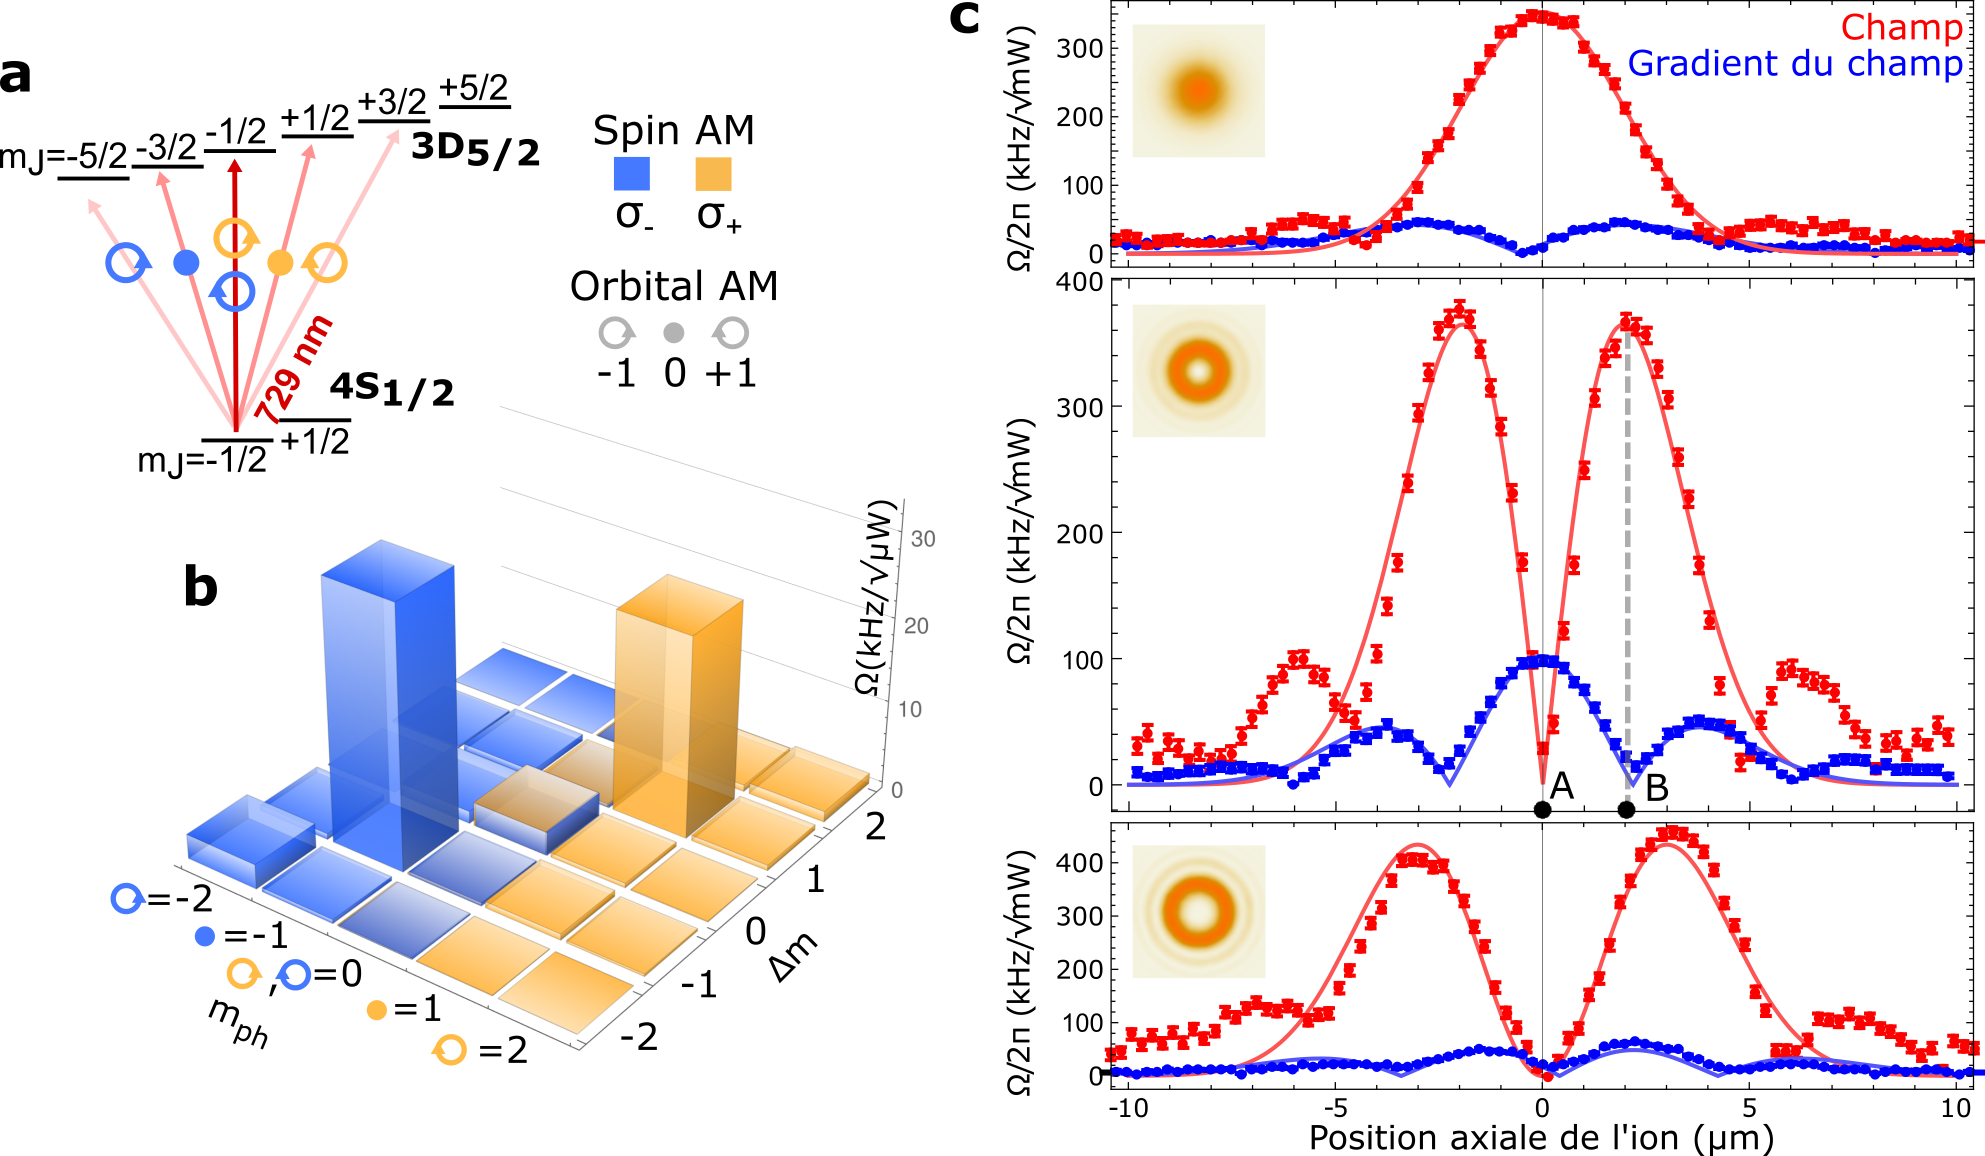
\includegraphics[width=0.9\columnwidth]{Figures/schmiegelow.png}
\caption{Observation de transition quadripolaire. (a) Transitions possibles mettant en jeu le MAS et le MAO. (b) Amplitudes de transition mesurées en utilisant une oscillation de Rabi. (c) Amplitude de transition dipolaire (rouge) et quadripolaire (bleu) en fonction de la position transverse de l'ion. Ces amplitudes sont reliées respectivement à l'amplitude du champ et du gradient du champ.}
\label{Fig:Schmiegelow}
\end{figure}


Nous avons maintenant terminé cette partie sur le concept de moment angulaire de la lumière. Nous avons introduit les définitions nécessaires et construit des champs électromagnétiques réalisables en pratiques dans lesquelles le moment angulaire est contrôlé. Dans le chapitre III, nous étudierons expérimentalement la génération de modes de Laguerre-Gauss à partir d'un laser infrarouge Gaussien, avant d'utiliser ces modes pour générer des harmoniques d'ordre élevé. Dans le chapitre IV, nous nous intéresserons au cas du moment angulaire de spin, c'est-à-dire de faisceaux polarisés circulairement. Nous chercherons à générer des harmoniques d'ordre élevé polarisées circulairement et à les utiliser dans l'étude de molécules chirales.